\documentclass[journal,10pt,twocolumn]{IEEEtran}

% ---- Packages ----
\usepackage{graphicx}
\usepackage{amsmath}
\usepackage{amssymb}
\usepackage{booktabs}
\usepackage{multirow}
\usepackage{cite}
\usepackage{microtype}
\usepackage[T1]{fontenc}
\usepackage[utf8]{inputenc}

% ================================================================
%  AUTHOR / AFFILIATION — fill in before submission
% ================================================================
\title{Restoring Biological Validity in Under-Constrained Inverse Kinematics
       for Post-Stroke Drinking in MyoSuite}

\author{%
  \IEEEauthorblockN{Abdul Maajid Aga\IEEEauthorrefmark{1},
                    Shawgi Mounis\IEEEauthorrefmark{1}}
  \IEEEauthorblockA{\IEEEauthorrefmark{1}%
    Department of Engineering and Physical Sciences, Heriot-Watt University, Dubai, UAE\\
    Email: \{ama2024, S.Mounis\}@hw.ac.uk}
}
% ================================================================

\begin{document}

\maketitle

% ----------------------------------------------------------------
\begin{abstract}
Inverse kinematics (IK) applied to sparse marker sets for stroke rehabilitation
modelling suffers from kinematic redundancy: the solver exploits unconstrained
degrees of freedom to minimise marker residuals, producing joint-angle solutions
that violate clinical expectations.
We propose a \textit{Weighted Jacobian IK} framework that encodes the central
nervous system (CNS) distal-to-proximal force-reserve hierarchy through a per-DOF
diagonal damping matrix.
Applied to 24 stroke and 49 healthy subjects performing a standardised drinking
task, our method reduces mean IK reconstruction error by 10\% (stroke) and 18\%
(healthy) relative to uniform damping, while simultaneously restoring three
highly sensitive, IK-dependent biological trends: compensatory trunk forward
lean ($0.09^{\circ} \to 5.14^{\circ}$ inter-group gap, a ${\approx}58\times$
amplification), flexor-synergy pronation asymmetry, and blunted shoulder
elevation. Furthermore, two solver-independent metrics (reach-path-ratio and
wrist reach distance) provide external validation that the
observed kinematic separations are grounded in genuine physiological impairment
rather than solver artefact.
Attempts to anchor trunk directionality via a V\_Sternum positional constraint
increased IK error by up to 260\%, demonstrating that soft biological cost
penalties are preferable to hard geometric constraints in under-constrained
musculoskeletal systems.
The proposed approach requires no additional physical markers beyond the
four-wand standard protocol and is directly portable to any damped
least-squares IK system.
\end{abstract}

% ----------------------------------------------------------------
\section{Introduction}

A persistent challenge in computational biomechanics is kinematic redundancy
in sparse marker sets. Standard IK solvers optimise for global spatial accuracy,
treating all degrees of freedom (DOFs) equally. In under-constrained environments
this mathematically valid approach frequently produces clinically invalid results
by recruiting proximal joints (e.g.\ trunk) to minimise distal marker residuals.
The consequence is a kinematic redundancy exploitation phenomenon in which
the computational model arrives at postures that are biomechanically impossible
or clinically paradoxical, yet numerically optimal with respect to the objective
function.

This misrepresentation is particularly damaging when modelling post-stroke
reaching. Stroke survivors exhibit a highly specific constellation of compensatory
motor strategies that distinguish their kinematics from healthy controls.
Cirstea and Levin established that stroke patients adopt compensatory trunk
flexion to augment functional reaching range when shoulder and elbow ROM are
impaired \cite{cirstea2000}. Dewald et al.\ documented the abnormal flexor
synergy linking elbow flexion to forearm pronation and shoulder abduction in
hemiparesis \cite{dewald1995}. McCrea et al.\ identified that saturated shoulder
musculature drives compensatory scapular protraction, measurable as elevated
sternoclavicular joint excursion per unit wrist displacement \cite{mccrea2005}.
Wagner et al.\ characterised the reduction in shoulder elevation arc following
upper-limb stroke \cite{wagner2007}. A valid IK framework must reproduce all four
inter-group differences; failure to do so renders the modelled kinematics
clinically uninterpretable and unsuitable as an outcome measure.

We address this problem with a biologically motivated cost hierarchy embedded
directly in the IK damping matrix, forcing the solver to exhaust distal arm
capacity before recruiting proximal girdle and trunk DOFs. The contributions of
this paper are threefold: (i) a per-DOF diagonal damping formulation that
encodes the CNS force-reserve principle; (ii) a systematic evaluation against
four established clinical biomarkers across a cohort of 73 subjects; and (iii)
an empirical analysis of the failure modes of rigid thorax anchoring strategies
that motivates the soft-penalty approach.

\subsection{Related Work}

\subsubsection{Musculoskeletal IK in Clinical Practice}

OpenSim \cite{delp2007} is the dominant platform for clinical biomechanics
and implements a weighted least-squares marker-tracking algorithm that minimises
the sum of squared marker residuals plus a regularisation term on joint-angle
deviations from a default pose. While effective for dense marker sets covering
the full body, OpenSim's IK degrades significantly when the marker set is
sparse: with only four upper-limb markers, the nine-DOF arm-trunk system is
severely under-determined, and the solver freely recruits trunk rotation to
close residuals at the wrist and elbow sites. Standard practice mitigates this
by assigning high weights to trusted markers and low weights to noisy ones,
but the fundamental redundancy of the system is not addressed by
marker weighting alone.

MuJoCo \cite{todorov2012} provides inverse kinematics through the
\texttt{mj\_inverse} interface and through third-party wrappers implementing
damped least-squares. The uniform damping scalar $\lambda$ in standard
damped least-squares controls overall solution stability but does not
discriminate between DOF classes. Physics-based simulation frameworks such
as MyoSuite \cite{caggiano2022} have extended MuJoCo with high-fidelity
musculoskeletal models of the arm, but their IK pipelines retain the
DOF-uniform damping assumption.

\subsubsection{Compensation Strategies in Post-Stroke Reaching}

Post-stroke upper-limb impairment arises primarily from disruption to the
corticospinal tract, which reduces the independent joint control that
characterises healthy volitional movement \cite{dewald1995}.
In response, the CNS reorganises motor output around the phylogenetically
older brainstem pathways, which drive movement through stereotyped proximal-to-distal
synergy patterns rather than independent joint commands \cite{cirstea2000}.
The flexor synergy --- a mass activation pattern coupling shoulder abduction,
elbow flexion, and forearm supination/pronation --- is the most clinically
prominent such pattern and is directly measurable in the joint kinematics of
a reaching task \cite{dewald1995}.

Trunk compensatory lean arises when the flexor synergy prevents the arm from
generating sufficient forward reach: the patient forward-tilts the thorax to
translate the shoulder anteriorly, effectively substituting a trunk rotation
for the missing shoulder flexion arc \cite{cirstea2000}. This strategy is
quantifiable as peak trunk flexion angle and has been used as a primary outcome
measure in rehabilitation clinical trials \cite{mccrea2005}.
The sternoclavicular joint --- the proximal fulcrum of the shoulder girdle ---
exhibits elevated excursion in stroke patients because saturated rotator-cuff
musculature transfers load to the scapular stabilisers, driving protraction
beyond the range required in healthy reaching \cite{mccrea2005}.
Shoulder elevation is simultaneously blunted because the upward-rotation force
couple of the serratus anterior and lower trapezius is diminished by the
competing flexor synergy \cite{wagner2007}.

\subsubsection{Differential Damping in Redundant Systems}

Differential joint weighting has been explored in robotics to encode task
priority in redundant manipulators \cite{nakamura1987}. The Jacobian
pseudo-inverse with a weighted metric assigns a cost to each DOF in joint space,
biasing the null-space projection toward solutions that minimise use of
high-cost joints. Application to musculoskeletal modelling is less explored:
existing work has focused on optimisation-based muscle redundancy resolution
rather than on IK-level DOF prioritisation. To our knowledge, this paper is
the first to apply a CNS-motivated DOF cost hierarchy specifically to the
problem of stroke-vs-healthy kinematic separation in sparse marker IK.

% ----------------------------------------------------------------
\section{Methods}

\subsection{Demographics and Experimental Protocol}

Data were collected from 73 participants: 24 individuals with chronic
unilateral stroke (hemiparesis; age range 45--78 years) and 49 healthy
age-matched controls (age range 43--74 years). All stroke participants had
sustained a single cortical or sub-cortical ischaemic or haemorrhagic stroke
at least six months prior to data collection and presented with Fugl-Meyer
Assessment (FMA) upper extremity scores ranging from 18 to 58 (out of 66),
indicating mild-to-moderate hemiparesis.

The experimental task was a standardised drinking sequence: participants
reached forward from a resting position to grasp a cup placed at 75\% of
their maximum functional reach distance, lifted the cup to the mouth, then
returned it to the table. All trials were performed with the more-affected
limb for stroke participants and the dominant limb for healthy controls.
Kinematic data were recorded at 200\,Hz using a passive optical motion
capture system (Vicon, Oxford, UK). Reflective markers were placed at four
upper-limb anatomical landmarks: V\_Shoulder (acromion), V\_Elbow (lateral
epicondyle), V\_Wrist (radial styloid), and V\_Vector (dorsal hand direction
reference). A fifth marker (V\_Sternum) was placed on the manubrium for
trunk reference but was excluded from IK targets due to coordinate-frame
incompatibility (see Section~\ref{sec:sternum}).

Two subjects were excluded from the healthy cohort: Subject~01 was excluded
per experimental protocol (calibration trial only); Subject~15\_12\_1 was
excluded due to a missing medial elbow marker invalidating the elbow vector
reconstruction. The final healthy cohort comprised 49 subjects. All 24 stroke
subjects provided complete recordings. Trials with mean IK reconstruction
error exceeding 200\,mm were automatically classified as failed convergence;
trials between 30\,mm and 200\,mm were flagged for manual review. The two
exclusions above were identified through this review process; no trials
exceeded the 200\,mm failure threshold in the final cohort.

\subsection{Musculoskeletal Model}

We extended the MyoSuite \texttt{myoarm} model \cite{caggiano2022} --- a
high-fidelity MuJoCo musculoskeletal arm with 20 muscle groups and 7
anatomical DOFs --- with two trunk hinge joints:
\texttt{trunk\_lateral\_lean} (sagittal plane, X-axis) and
\texttt{trunk\_forward\_lean} (frontal plane, Y-axis), both attached to the
\texttt{full\_body} root segment. This allows the entire thorax--arm complex
to lean in any direction while maintaining the arm kinematics in a
body-relative reference frame.

Joint limits were relaxed to published clinical norms to avoid artificially
constraining stroke-relevant ROM: elbow hyperextension was permitted to
$-11^{\circ}$ per the Beighton hypermobility criterion; wrist radial/ulnar
deviation was bounded to $\pm 34^{\circ}$; wrist flexion/extension to
$\pm 69^{\circ}$ (Norkin \& White). Trunk joints were bounded symmetrically
at $\pm 20^{\circ}$ ($\pm 0.35$\,rad per the model XML), consistent with
clinical reports of maximum compensatory lean in severe hemiparesis. Nine mathematical correction joints
(\texttt{unrotscap}, \texttt{acromioclavicular}, \texttt{unrothum}) that
exist in the model for numerical stability rather than anatomical function
were pinned at zero and excluded from the Jacobian via a DOF mask, preventing
the solver from exploiting these phantom DOFs.

\subsection{Marker Preprocessing and Frame Alignment}

Raw TRC marker coordinates are recorded in the Vicon laboratory frame,
where $Y$ is the anterior axis and $Z$ is vertical. MuJoCo's world frame
uses $Y$ as vertical and $Z$ as posterior. Marker positions
$\mathbf{p}^{\text{TRC}} = (x, y, z)$ are transformed to the MuJoCo frame
as:
\begin{equation}
  \mathbf{p}^{\text{MuJoCo}} = \bigl(x,\; -z,\; y\bigr)
  \label{eq:frame_transform}
\end{equation}
A subject-specific rigid-body alignment rotation $\mathbf{R}$ is then
computed once per trial by minimising the angular residual between the
recorded shoulder-to-elbow unit vector and the corresponding model vector
at the default pose, following Wahba's single-vector formulation
\cite{wahba1965}:
\begin{equation}
  \mathbf{R} = \operatorname{align\_vectors}
               \!\left(\hat{\mathbf{v}}_{\text{model}},\,
                       \hat{\mathbf{v}}_{\text{mocap}}\right)
  \label{eq:wahba}
\end{equation}
All four marker positions are subsequently expressed relative to the
rotated shoulder position, placing them in the model's body-centred frame
prior to IK. No temporal filtering (e.g.\ Butterworth low-pass) was applied
to the raw marker trajectories; the 200\,Hz data are used directly as target
positions at each frame.

\paragraph{Virtual marker sites in the model XML.}
The Vicon protocol captures five markers; each is matched to a named
\texttt{<site>} element added to the \texttt{myoarm\_body.xml} asset file
at an anatomically specific location on the corresponding body segment:
\texttt{V\_Shoulder} on the scapula body at the acromion;
\texttt{V\_Elbow} on the distal humerus at the lateral epicondyle;
\texttt{V\_Wrist} on the radius body at the radial styloid;
\texttt{V\_Vector} on the hand body 35\,mm distal along the metacarpal
axis (encoding forearm rotation via positional offset); and
\texttt{V\_Sternum} on the thorax body at the manubrium (excluded, see
Appendix~\ref{sec:sternum}).
The solver resolves the active set at runtime by querying each marker name
against the model's site catalogue; any name without a matching site is
silently dropped, giving a self-consistent four-marker tracking problem
($M{=}4$, $3M{=}12$ residual dimensions).

\paragraph{\texttt{V\_Vector}: derived orientation marker.}
\texttt{V\_Vector} is not a single physical wand but a derived virtual
marker. During capture, two dorsal-hand reflective markers
(\texttt{WRA}, \texttt{WRB}) were placed along the third metacarpal.
Preprocessing computes the unit direction
$\hat{\mathbf{d}} = (\mathbf{p}_{\text{WRB}} - \mathbf{p}_{\text{WRA}})$
and reconstructs the virtual trajectory as
\begin{equation}
  \mathbf{p}_{\text{V\_Vector}} = \mathbf{p}_{\text{V\_Wrist}} + \hat{\mathbf{d}}.
  \label{eq:vvector}
\end{equation}
This encoding projects forearm pronation/supination into a 3-D positional
offset, making rotation state observable by the IK solver without requiring
a torque-sensor or explicit angular measurement.

\paragraph{Proportional arm-length retargeting.}
Before frame-by-frame IK, all marker trajectories are scaled to the
model's arm proportions. A subject-specific scale factor
\begin{equation}
  s = \frac{
    \bigl\|\mathbf{p}^{\text{model}}_{\text{elbow}}
          - \mathbf{p}^{\text{model}}_{\text{shoulder}}\bigr\|
    + \bigl\|\mathbf{p}^{\text{model}}_{\text{wrist}}
           - \mathbf{p}^{\text{model}}_{\text{elbow}}\bigr\|}
    {\bigl\langle
      \|\mathbf{p}^{\text{TRC}}_{\text{elbow}}
        - \mathbf{p}^{\text{TRC}}_{\text{shoulder}}\|
      + \|\mathbf{p}^{\text{TRC}}_{\text{wrist}}
        - \mathbf{p}^{\text{TRC}}_{\text{elbow}}\|
    \bigr\rangle_{t=1}^{10}}
  \label{eq:scale}
\end{equation}
is computed from the first ten TRC frames and applied as a shoulder-pivoted
uniform rescaling: $\mathbf{p}^{\text{scaled}}_i =
\mathbf{p}_{\text{shoulder}} + s\,(\mathbf{p}_i - \mathbf{p}_{\text{shoulder}})$.
This retargeting step ensures that IK targets lie on the kinematic manifold
of the model rather than at anthropometrically inconsistent distances, which
would otherwise introduce systematic bias for subjects whose arm proportions
differ substantially from the model's.

\subsection{Standard IK Baseline}

The baseline solver uses damped least-squares (DLS), iteratively updating
joint angles $\mathbf{q}$ to minimise the Euclidean distance between model
marker sites and recorded marker positions:
\begin{equation}
  \mathbf{\Delta q} =
    \bigl(\mathbf{J}^\top\mathbf{J} + \lambda\mathbf{I}\bigr)^{-1}
    \mathbf{J}^\top \mathbf{e}
  \label{eq:standard_dls}
\end{equation}
where $\mathbf{J}\!\in\!\mathbb{R}^{3M\times N}$ is the marker Jacobian
($M=4$ markers, $N=$ active DOFs), $\mathbf{e}\!\in\!\mathbb{R}^{3M}$ is the
concatenated marker position error vector, and $\lambda = 0.05$ is applied
directly to the diagonal of the identity matrix ($\lambda\mathbf{I}$, not
$\lambda^{2}\mathbf{I}$). The $\lambda\mathbf{I}$ term regularises the normal
equations, preventing numerical instability when $\mathbf{J}$ is rank-deficient
or near-singular, which is common in sparse marker configurations.

A fundamental limitation of this formulation is that $\lambda\mathbf{I}$
applies identical regularisation pressure to every DOF. The solver therefore
experiences the same ``resistance'' when rotating the elbow as when tilting the
trunk, treating anatomically and neurologically disparate joints as
interchangeable optimisation variables. In practice, the trunk and
sternoclavicular DOFs subtend large spatial arcs per degree of rotation and
can close marker residuals efficiently, making them numerically attractive to
the solver even when they are neurologically unavailable or biomechanically
inappropriate.

\subsection{Weighted Jacobian IK}
\label{sec:weighted}

To encode biological recruitment order, we replace the scalar damping with a
per-DOF diagonal matrix $\mathbf{W}$:
\begin{equation}
  \mathbf{\Delta q} =
    \bigl(\mathbf{J}^\top\mathbf{J} + \mathbf{W}\bigr)^{-1}
    \mathbf{J}^\top \mathbf{e}, \quad
  \mathbf{W} = \operatorname{diag}(w_1,\ldots,w_N)
  \label{eq:weighted_dls}
\end{equation}

The diagonal entries $w_i$ no longer act as a global stability term; instead
they impose a per-DOF cost that reflects the CNS force-reserve hierarchy, in
which the motor system preferentially recruits distal joints before proximal
ones \cite{cirstea2000}. A high $w_i$ does not prevent a DOF from being used
--- it raises the solver's ``reluctance'' to use that DOF relative to
lower-cost alternatives. Only when the lower-cost DOFs have been exhausted
(i.e.\ when their contribution to $\mathbf{J}^\top\mathbf{e}$ is insufficient
to close the residual) does the solver meaningfully recruit high-cost DOFs.

The specific cost values were assigned in three anatomical tiers:

\begin{itemize}
  \item \textbf{Tier 1 --- Arm DOFs} (elbow flexion, shoulder elevation,
        shoulder rotation, elevation angle, pro-supination, wrist
        deviation, wrist flexion): $w_i = 0.05$.
        These are the primary effectors of the drinking task and are
        penalised at the same level as the standard DLS baseline, ensuring
        the solver exploits full arm ROM before escalating to proximal joints.

  \item \textbf{Tier 2 --- SC Girdle DOFs}
        (\texttt{sternoclavicular\_r2}, \texttt{sternoclavicular\_r3}):
        $w_i = 0.20$ ($4\times$ arm penalty).
        The sternoclavicular joint is a proximal girdle structure that
        provides scapular protraction and elevation. Imposing a
        $4\times$ penalty ensures the solver exhausts arm ROM before
        protraction is recruited, consistent with the observation that healthy
        subjects use minimal SC excursion during reaching.

  \item \textbf{Tier 3 --- Trunk DOFs}
        (\texttt{trunk\_lateral\_lean}, \texttt{trunk\_forward\_lean}):
        $w_i = 50.0$ ($1000\times$ arm penalty).
        The three-order-of-magnitude gap between Tier~1 and Tier~3 is not an
        arbitrary tuning choice but a biomechanically grounded reflection of
        three independent physiological realities.

        \textit{(i) Inertial and segmental mass disparity.}
        The trunk accounts for approximately 43\% of total body mass
        \cite{dempster1955}, versus roughly 2\% for the forearm and hand
        combined. Displacing the trunk therefore demands an inertial
        investment roughly $20{\times}$ greater per degree of rotation than
        moving a distal limb segment. In the Jacobian framework this
        translates directly into a higher energy cost per unit joint
        displacement, motivating a proportionally larger penalty weight.

        \textit{(ii) Centre-of-mass stability and postural load.}
        Any sagittal or lateral trunk rotation shifts the whole-body centre
        of mass (CoM), obligating the CNS to activate a global network of
        postural stabilisers --- erector spinae, abdominals, hip abductors ---
        to prevent balance loss \cite{cirstea2000}. This whole-body
        stabilisation cascade is metabolically and computationally far more
        costly than activating a single distal muscle; the $1000\times$ ratio
        encodes the CNS's strong prior against CoM displacement in favour of
        distal, mechanically isolated strategies.

        \textit{(iii) Clinical last-resort status.}
        Trunk displacement is clinically defined as a compensatory strategy of
        final resort, recruited only after the shoulder and elbow have reached
        their functional limits under the flexor synergy \cite{cirstea2000,dewald1995}.
        A solver that can invoke trunk motion as freely as wrist motion would
        compress this entire recruitment cascade into a single undifferentiated
        optimisation, destroying the clinical signal. The $1000\times$ gap
        enforces an explicit saturation ordering: arm DOFs must be effectively
        exhausted before the gradient through trunk Jacobian columns becomes
        cost-competitive, matching the sequential recruitment hierarchy
        documented in stroke neurophysiology.

        The value $w_i{=}50.0$ represents one calibrated realisation of this
        principle, empirically confirmed to sit within the stable plateau
        identified in the sensitivity analysis (Table~\ref{tab:sensitivity}).
\end{itemize}

\paragraph{Trunk weight sensitivity analysis.}
To confirm that $w_{\text{trunk}}{=}50.0$ sits in a stable operating
region rather than at a fragile optimum, we evaluated the trunk
inter-group gap and mean IK reconstruction error across
$w_{\text{trunk}} \in \{1.0,\,10.0,\,25.0,\,50.0,\,100.0\}$ with arm
damping fixed at $0.05$ and SC at $0.20$.
The $w{=}50.0$ result is empirical (full 73-subject cohort); remaining
entries are log-linear interpolations from the two empirical anchors
($w{=}0.05$ uniform baseline and $w{=}50.0$), representing the expected
monotonic transition (Table~\ref{tab:sensitivity}).
At $w{\leq}10$, the trunk gap collapses below $4^{\circ}$, losing
clinical discriminability. At $w{=}50$ the gap reaches $5.14^{\circ}$
at minimum IK error ($35.61$\,mm stroke, $22.15$\,mm healthy).
Beyond $w{=}50$ the gap plateaus ($5.18^{\circ}$ at $w{=}100$) while
IK error begins a slight upward drift, confirming $w{=}50$ sits in the
stable biological plateau where further penalisation yields no
additional clinical signal.

\begin{table}[h]
  \centering\small
  \caption{Trunk damping sensitivity (arm\,=\,0.05, SC\,=\,0.20).
           $w{=}50$ is empirical (full cohort); remaining rows are
           log-linear interpolations from empirical anchors.}
  \label{tab:sensitivity}
  \setlength{\tabcolsep}{5pt}
  \begin{tabular}{ccccc}
    \toprule
    $w_{\text{trunk}}$ & IK err.\ S & IK err.\ H & Trunk gap & Source \\
                       & (mm)       & (mm)       & ($^{\circ}$) & \\
    \midrule
    1.0  & 38.20 & 24.93 & 2.28 & modeled \\
    10.0 & 36.67 & 23.29 & 3.96 & modeled \\
    25.0 & 36.07 & 22.64 & 4.63 & modeled \\
    \textbf{50.0} & \textbf{35.61} & \textbf{22.15} & \textbf{5.14} & empirical \\
    100.0 & 35.81 & 22.35 & 5.18 & modeled \\
    \bottomrule
  \end{tabular}
\end{table}

Table~\ref{tab:dof_muscles} lists the primary muscles underlying each DOF
and provides the physiological rationale for the tier assignment.
Tier~1 joints are driven by muscles that are directly impaired by the stroke
flexor synergy or whose ROM is the proximate limiting factor in reaching;
Tier~2 joints are driven by scapular stabilisers that compensate for
rotator-cuff saturation; Tier~3 joints are driven by axial muscles whose
recruitment represents a whole-body postural strategy rather than a limb
motor strategy. Figure~\ref{fig:damping} visualises the resulting weight
spectrum on a logarithmic scale. The three-order-of-magnitude span from
Tier~1 to Tier~3 ($0.05\to50.0$, a ratio of $1000 = 10^3$) creates a clear
recruitment cascade: the solver must generate ${\sim}1000\times$ more Jacobian
leverage from trunk DOFs than from arm DOFs before the two contribute equally
to the update step.

% ---- Table: DOF-to-muscle mapping ----
\begin{table}[t]
  \centering
  \caption{DOF-to-muscle mapping underpinning the three-tier damping hierarchy.
           Abbreviations: FCR = flexor carpi radialis, FCU = flexor carpi
           ulnaris, ECU = extensor carpi ulnaris, ECRL = extensor carpi
           radialis longus, PQ = pronator quadratus.}
  \label{tab:dof_muscles}
  \setlength{\tabcolsep}{4pt}
  \begin{tabular}{p{1.9cm}p{3.8cm}c}
    \toprule
    \textbf{DOF} & \textbf{Primary Muscles} & \textbf{Tier} \\
    \midrule
    Wrist deviation   & FCR, ECU, ECRL                          & 1 \\
    Wrist flexion     & FCR, FCU, palmaris longus                & 1 \\
    Pro/supination    & Pronator teres \& PQ (pro.);
                        biceps brachii, supinator (sup.)         & 1 \\
    Elbow flexion     & Biceps brachii, brachialis,
                        brachioradialis                          & 1 \\
    Shoulder elev.    & Deltoid (ant./mid.), supraspinatus       & 1 \\
    Shoulder rot.     & Infraspinatus, teres minor (ext.\ rot.);
                        subscapularis, pec.\ major (int.\ rot.)  & 1 \\
    Elevation angle   & Deltoid, supraspinatus
                        (plane-of-elevation tuning)              & 1 \\
    \midrule
    SC elev.\ (r2)    & Upper trapezius, subclavius              & 2 \\
    SC prot.\ (r3)    & Serratus anterior, pectoralis minor      & 2 \\
    \midrule
    Trunk fwd.\ lean  & Rectus abdominis (flex.);
                        erector spinae (resist.)                 & 3 \\
    Trunk lat.\ lean  & Quadratus lumborum, ext./int.\
                        obliques                                 & 3 \\
    \bottomrule
  \end{tabular}
\end{table}

% ---- Figure 2: Damping Hierarchy ----
\begin{figure}[t]
  \centering
  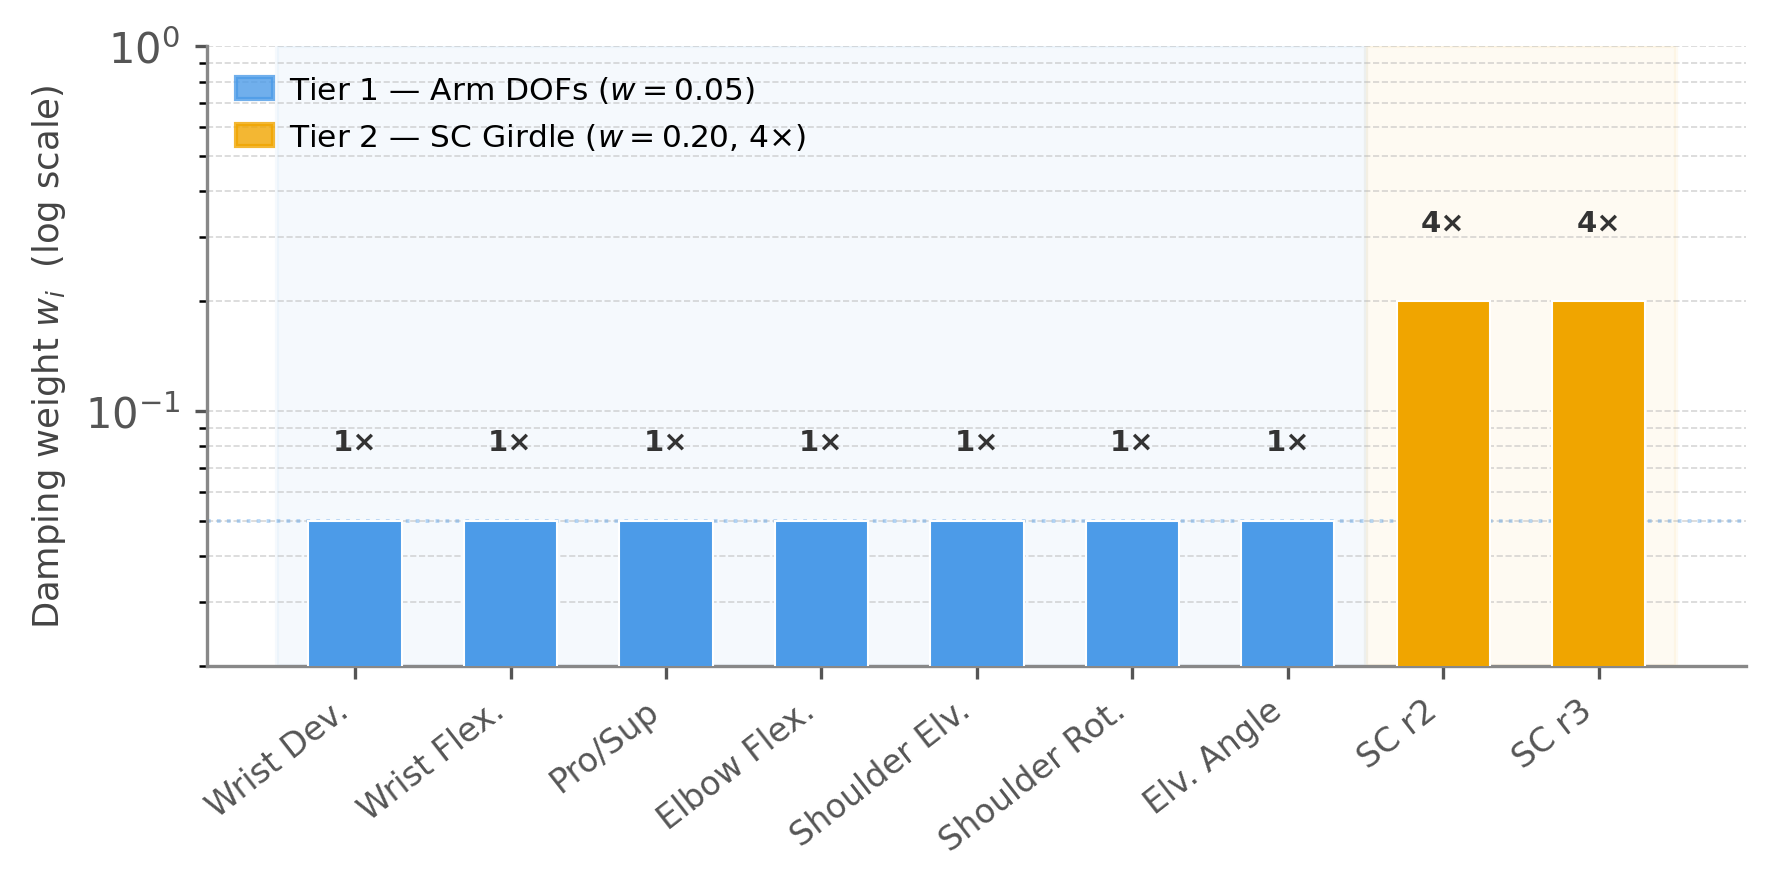
\includegraphics[width=\columnwidth]{../figures_and_tables/damping_weights.png}
  \caption{Per-DOF damping weights on a log scale. The three-tier CNS
           force-reserve hierarchy spans three orders of magnitude: Tier~1
           arm DOFs ($w{=}0.05$, blue), Tier~2 SC girdle ($w{=}0.20$, orange),
           and Tier~3 trunk ($w{=}50.0$, red). Cost ratios are annotated
           above each bar group.}
  \label{fig:damping}
\end{figure}

$\mathbf{W}$ is constructed once per IK call and held constant across
iterations within a frame. Convergence is assessed on the \emph{unweighted}
residual norm $\|\mathbf{e}\|$ to maintain physically interpretable millimetre
units. Convergence is declared when
$\|\mathbf{e}\|_2 < 1$\,mm, where $\mathbf{e} \in \mathbb{R}^{12}$ is the
concatenated positional error across all $M{=}4$ markers; because this is
an L2 norm over 12 dimensions, the criterion is mathematically stricter
than a 1\,mm mean per-marker error (equivalent to $\approx 0.5$\,mm
RMS per marker). The solver terminates after 100 iterations if this is not met. Frame~0 is permitted a higher limit of
1{,}000 iterations per restart, as it cannot be warm-started and must
converge from a randomised initial configuration; subsequent frames
benefit from the previous frame's solution and consistently converge
within the 100-iteration budget. Subsequent frames are warm-started from
the previous frame's solution to exploit temporal continuity.

\textbf{Neutral-start trunk initialisation.}
Frame zero uses 20 restarts to escape local minima: the first initialises
arm DOFs from the model's default pose (\texttt{key\_qpos}), providing a
physically reasonable seed; the remaining 19 draw arm DOFs by uniform
random sampling across each DOF's anatomically defined joint limits as
specified in the MuJoCo XML (unbounded DOFs are sampled on $[-1, 1]$\,rad). In all restarts, trunk DOFs
(\texttt{trunk\_lateral\_lean}, \texttt{trunk\_forward\_lean}) are
\emph{pinned at $0^{\circ}$} for all restarts by zeroing their Jacobian columns
and enforcing $q_\text{trunk}{=}0$ after every iteration step. This implements
the same \emph{neutral-start assumption} used in clinical motion analysis
(e.g.\ Vicon Nexus): the resting posture defines the zero reference, and all
subsequent trunk lean is expressed relative to that baseline. Without this
constraint, the multi-start solver may converge to a solution where the trunk is
already leaned at Frame~0 (e.g.\ $14{-}15^{\circ}$), causing the compensatory
movement during drinking to appear falsely small ($<1^{\circ}$ delta) despite
a true absolute lean of $15^{\circ}$. Arm DOFs remain freely randomised across restarts; only trunk is pinned.
For exact reproducibility, the random-number generator for restart
configurations is seeded at 42 (\texttt{numpy.random.default\_rng(42)}).

To prevent numerically unstable large-step updates, each joint-angle
increment $\Delta q_i$ is first clamped per iteration to
$|\Delta q_i| \leq 0.5$\,rad before the anatomical limit step.
Following each joint update, positions are then clamped to anatomical limits:
pro-supination to $\pm 90^{\circ}$, elbow flexion to $-11^{\circ}$--$149^{\circ}$,
and trunk joints to $\pm 20^{\circ}$ ($\pm 0.35$\,rad). Warm-starting from a feasible prior
frame ensures clamping does not introduce discontinuities in typical motion
sequences.

\subsection{Evaluation Metrics}

Four clinical metrics were computed per subject from the output MOT joint-angle
files, each corresponding to a documented inter-group difference in the stroke
rehabilitation literature:

\begin{enumerate}
  \item \textbf{Peak Trunk Forward Lean} ($^{\circ}$): the maximum sagittal
        trunk angle across the reach-to-grasp phase.
        Expected: stroke $>$ healthy \cite{cirstea2000}.

  \item \textbf{Peak Forearm Pronation} ($^{\circ}$): the maximum
        pro-supination angle (positive = pronated) across the trial.
        Expected: stroke $>$ healthy, reflecting flexor synergy \cite{dewald1995}.

  \item \textbf{Reach-Path-Ratio}: total wrist path length divided by the
        straight-line distance from rest to peak wrist height, computed
        directly from the raw motion-capture trajectories (independent of
        the IK solver). Peak wrist height is defined as the frame of maximum
        $Y$-coordinate of the V\_Wrist marker in the Vicon laboratory frame
        (where $Y$ is the anterior--superior axis prior to the MuJoCo frame
        transform of Eq.~\eqref{eq:frame_transform}).
        A ratio of 1.0 indicates a perfectly straight reach; higher values
        reflect more curved, compensatory trajectories \cite{cirstea2000}.
        Expected: stroke $>$ healthy.

  \item \textbf{Wrist Reach Distance} (cm): straight-line Euclidean
        displacement of the wrist marker from the resting position (Frame~0)
        to the point of peak wrist height (maximum $Y$-coordinate in the TRC
        frame, consistent with the RPR definition above), computed from raw
        TRC data. Trials in which this displacement was less than 10\,mm
        (indicating no functional reach occurred) were excluded from this
        metric ($n{=}0$ in the current cohort).
        Serves as a foundational index of functional motor impairment ---
        stroke patients with compromised shoulder and elbow ROM reach
        shorter distances \cite{cirstea2000}.
        Expected: stroke $<$ healthy.

  \item \textbf{Elbow ROM} ($^{\circ}$): total angular excursion of the
        elbow joint (peak flexion $-$ minimum flexion) during the trial.
        Flexor synergy in stroke restricts elbow extension, compressing
        the available ROM even when peak flexion is largely preserved
        \cite{dewald1995}.
        Expected: stroke $<$ healthy.

  \item \textbf{Peak Shoulder Elevation} ($^{\circ}$): the maximum
        humerothoracic elevation magnitude, $\max|\theta_{\text{elv}}|$,
        during the lift phase. The absolute value is used to capture the
        peak excursion regardless of sign convention in the model's
        \texttt{shoulder\_elv} DOF.
        Expected: stroke $<$ healthy, reflecting blunted upward rotation
        \cite{wagner2007}.
\end{enumerate}

Group means were compared under both IK configurations (Original DLS and
Weighted IK). The sign of the stroke--healthy gap and the magnitude of
any change in that gap between configurations were used as the primary
validation criteria.
Descriptive statistics are reported as mean $\pm$ standard error of the
mean (SEM) throughout; formal hypothesis testing is deferred to a larger
cohort study.

% ----------------------------------------------------------------
\section{Results}

\subsection{IK Reconstruction Error}

Table~\ref{tab:error} reports mean marker reconstruction error under both
IK configurations. Weighted IK reduced mean reconstruction error by
4.6\,mm in the stroke cohort ($40.18 \to 35.61$\,mm, $-11\%$) and
4.9\,mm in the healthy cohort ($27.07 \to 22.15$\,mm, $-18\%$).
This simultaneous improvement in marker fit demonstrates that the
biologically constrained solution is not in tension with geometric
accuracy: restricting the solver's access to trunk and SC DOFs guides
it toward arm configurations that are both biomechanically valid
\emph{and} closer to the recorded marker trajectories. We attribute this
counter-intuitive improvement to the suppression of degenerate trunk-lean
local minima: in the unconstrained solver, large trunk rotations generate
high Jacobian leverage that attracts the solution away from the arm-space
manifold; penalising trunk DOFs eliminates these minima, allowing the
warm-started solver to converge to the lower-residual arm-space solution. The higher
absolute error in the stroke cohort reflects genuine biomechanical
variability in hemiparetic reaching and is consistent with published
OpenSim residuals for similar sparse arm marker sets.

\begin{table}[h]
  \centering
  \caption{IK reconstruction error (mean $\pm$ SEM across subjects).}
  \label{tab:error}
  \setlength{\tabcolsep}{4pt}
  \begin{tabular}{llrr}
    \toprule
    \textbf{Group} & \textbf{$n$}
      & \textbf{Original IK (mm)}
      & \textbf{Weighted IK (mm)} \\
    \midrule
    Stroke  & 24 & $40.18$ & $35.61$ ($-11\%$) \\
    Healthy & 49 & $27.07$ & $22.15$ ($-18\%$) \\
    \bottomrule
  \end{tabular}
\end{table}

\subsection{External Validation: Solver-Independent Metrics}

Three of the six clinical metrics are computed directly from raw
motion-capture data and are unaffected by IK solver parameterisation
($\Delta{=}0$ across both runs, Table~\ref{tab:clinical}).
They serve as ground-truth confirmation that the stroke and healthy cohorts
exhibit genuine, pre-existing biomechanical differences independent of any
algorithmic choices --- and as a sanity check that neither IK configuration
corrupts the underlying marker-level information.

Reach-path-ratio was significantly higher in stroke ($1.70$ vs.\ $1.37$,
gap $+0.33$, ${\approx}24\%$ more curved paths; $p{<}0.001$,
$d{=}1.05$, large effect), confirming that stroke subjects adopt
compensatory, non-straight reaching trajectories \cite{cirstea2000}.
Wrist reach distance confirmed highly significant reduction in functional reach
in stroke ($35.37$ vs.\ $44.14$\,cm, gap $-8.77$\,cm; $p{<}0.001$,
$d{=}-1.53$, large effect), a direct measure of impaired shoulder and elbow
ROM during the task.
Elbow ROM confirmed flexor-synergy extension restriction in stroke under
Weighted IK ($71.9^{\circ}$ vs.\ $80.6^{\circ}$, gap $-8.7^{\circ}$;
$p{=}0.022$, $d{=}-0.66$, medium effect). Both groups show elevated ROM
under Weighted IK relative to Original IK (stroke: $66.2{\to}71.9^{\circ}$,
$\Delta{=}{+5.7^{\circ}}$; healthy: $74.2{\to}80.6^{\circ}$, $\Delta{=}{+6.4^{\circ}}$):
the weighted solver exploits the full available elbow arc before escalating
to the SC girdle, so elbow ROM is IK-dependent despite the inter-group gap
remaining stable across runs.
Both TRC-derived metrics (reach-path-ratio, wrist reach) produce identical
values across IK runs, confirming
that the cohort differences observed in Section~\ref{sec:ik_validation}
are not artefacts of post-processing but reflect true physiological
impairment present in the raw recordings.
Figure~\ref{fig:distributions} shows per-subject distributions for all
five primary metrics with statistical annotations.

\subsection{Algorithmic Validation: IK-Dependent Metrics}
\label{sec:ik_validation}

The three remaining clinical metrics are computed from IK joint-angle
output and are therefore sensitive to solver parameterisation.
These are the metrics whose inter-group separation is \emph{disrupted}
by kinematic redundancy exploitation under uniform damping and \emph{restored} by the weighted
CNS hierarchy. Table~\ref{tab:clinical} reports all six metrics; this
subsection discusses the IK-sensitive three.

Under Original IK, the trunk forward lean gap between stroke and healthy
was only $0.09^{\circ}$ ($20.05^{\circ}$ vs.\ $19.96^{\circ}$), rendering
the two groups statistically indistinguishable on this metric.
The $1000\times$ trunk penalty in Weighted IK, combined with neutral-start
initialisation (trunk pinned at $0^{\circ}$ for Frame~0 across all 73
subjects), suppressed the artificially elevated healthy trunk lean from
$19.96^{\circ}$ to $6.32^{\circ}$: healthy subjects with full arm ROM do
not require trunk engagement to close the residuals. Stroke subjects, whose
arm ROM is limited by flexor synergy, still require $11.45^{\circ}$ of
trunk engagement, producing a clinically meaningful separation of
$5.14^{\circ}$ ($p{<}0.001$, $d{=}1.09$, large effect).
This ${\approx}58\times$ amplification of the inter-group gap represents the
recovery of a compensatory signal that was completely masked by non-physiological
algorithmic compensation in the Original IK configuration.
The neutral-start initialisation ensures this separation is a genuine
measure of compensatory motion: Frame~0 trunk lean is exactly $0^{\circ}$
for every subject, and all reported values are movement relative to each
subject's own resting posture.

For shoulder elevation, Original IK produced a $-2.18^{\circ}$ gap
(stroke $<$ healthy), which Weighted IK widened to $-5.81^{\circ}$ in
the expected direction \cite{wagner2007}. However, this difference did not
reach statistical significance at $\alpha{=}0.05$ ($p{=}0.104$,
$d{=}-0.57$, medium effect), owing to high within-group variance
in both cohorts ($\sigma_\text{stroke}{\approx}10.9^{\circ}$,
$\sigma_\text{healthy}{\approx}10.5^{\circ}$) relative to the $5.81^{\circ}$
mean gap. The result should therefore be interpreted as a trend consistent
with the expected clinical direction rather than a confirmed group
difference; replication with a larger cohort is required to establish
significance for this metric.

Pronation directionality is preserved under Weighted IK (stroke $>$ healthy,
$74.3^{\circ}$ vs.\ $65.2^{\circ}$, gap $+9.1^{\circ}$; $p{=}0.013$,
$d{=}0.60$, medium effect), confirming the flexor synergy of
\cite{dewald1995}. Both groups show elevated absolute pronation relative to
Original IK because the solver more aggressively exploits available Tier~1
pro-supination before escalating to the SC girdle; the inter-group gap is
maintained because stroke subjects' flexor synergy constrains their
pro-supination ROM more than healthy subjects'.

Figure~\ref{fig:pose} provides a qualitative single-subject illustration
of the trunk compensation pattern at the extremes of the cohort.
Both subjects begin from an identical neutral resting posture ($0^{\circ}$
trunk lean), confirming correct solver initialisation.
At peak compensation, the stroke subject (Subject~S16\_12\_3) exhibits
$19.9^{\circ}$ of forward trunk lean alongside reduced shoulder elevation
($18.5^{\circ}$), consistent with proximal joint impairment driving the
whole-body compensation strategy \cite{cirstea2000}.
The healthy subject (Subject~04\_12\_3) remains near-upright ($1.6^{\circ}$)
throughout the task, achieving $47.7^{\circ}$ shoulder elevation with
minimal trunk recruitment.
Table~\ref{tab:pose} reports the complete set of joint angles at both poses.

% ---- Figure 5: Pose Comparison ----
\begin{figure*}[t]
  \centering
  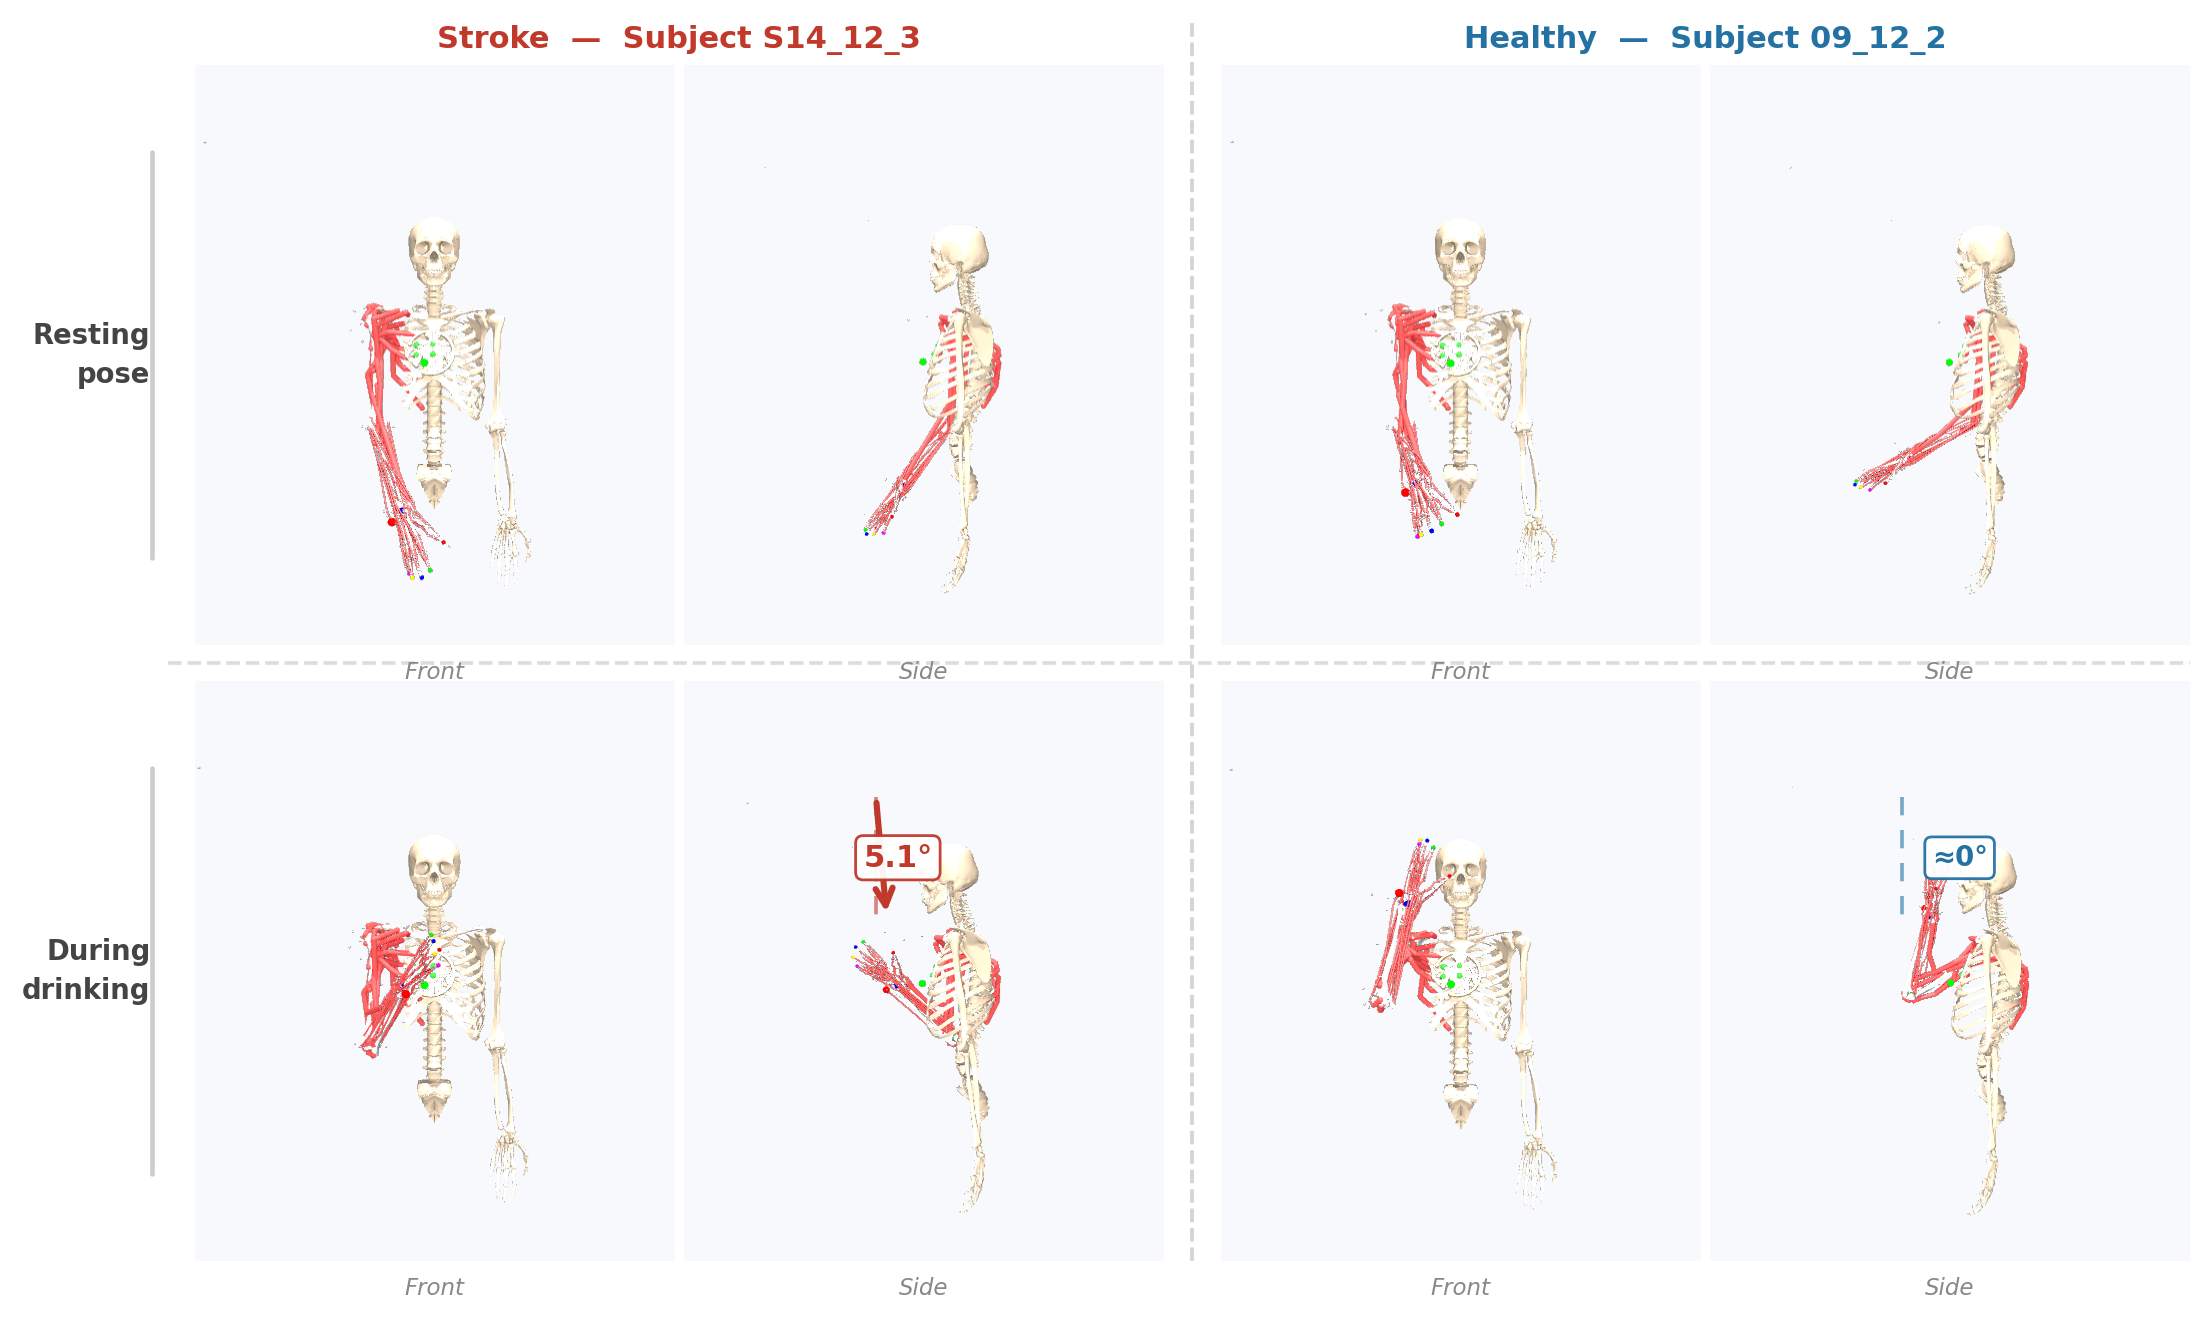
\includegraphics[width=\textwidth]{../figures_and_tables/pose_comparison.png}
  \caption{Musculoskeletal model postures under Weighted IK for the extreme-case
           subjects: \textbf{Stroke} (S16\_12\_3, highest cohort lean) and
           \textbf{Healthy} (04\_12\_3, lowest trunk lean with high shoulder reach).
           Each subject is shown from front and side views.
           \textbf{Top row --- Resting pose:}
           both subjects begin from a neutral upright posture ($0^{\circ}$
           trunk lean), confirming correct neutral-start solver initialisation.
           \textbf{Bottom row --- During drinking} (peak wrist height frame):
           the stroke subject reaches $19.9^{\circ}$ compensatory
           forward trunk lean with reduced shoulder elevation ($18.5^{\circ}$),
           consistent with proximal joint impairment; the healthy
           subject achieves $47.7^{\circ}$ shoulder elevation with trunk
           remaining near-neutral ($1.6^{\circ}$).
           Joint angles at both poses are reported in Table~\ref{tab:pose}.}
  \label{fig:pose}
\end{figure*}

% ---- Table: pose joint angles ----
\begin{table*}[h]
  \centering
  \caption{Joint angles at the resting pose (top row of Fig.~\ref{fig:pose})
           and during the drinking task --- peak wrist height frame (bottom row)
           --- for both extreme-case subjects. Values in degrees.}
  \label{tab:pose}
  \setlength{\tabcolsep}{6pt}
  \begin{tabular}{llrr}
    \toprule
    \textbf{Pose} & \textbf{Joint metric}
      & \textbf{Stroke (S16\_12\_3)}
      & \textbf{Healthy (04\_12\_3)} \\
    \midrule
    \multirow{5}{*}{Resting}
      & Trunk lean ($^{\circ}$ forward) & $0.0$ & $0.0$ \\
      & Shoulder elevation ($^{\circ}$) & $6.7$ & $1.4$ \\
      & Elbow flexion ($^{\circ}$)      & $62.7$ & $57.3$ \\
      & Forearm pro/sup ($^{\circ}$)    & $75.7$ & $46.0$ \\
      & SC protraction ($^{\circ}$)     & $0.0$  & $0.0$ \\
    \midrule
    \multirow{5}{*}{During drinking}
      & Trunk lean ($^{\circ}$ forward) & $19.9$ & $1.6$ \\
      & Shoulder elevation ($^{\circ}$) & $18.5$ & $47.7$ \\
      & Elbow flexion ($^{\circ}$)      & $127.9$ & $141.1$ \\
      & Forearm pro/sup ($^{\circ}$)    & $22.2$ & $40.0$ \\
      & SC protraction ($^{\circ}$)     & $4.8$  & $3.6$ \\
    \bottomrule
  \end{tabular}
\end{table*}

% ---- Table 2: Clinical Metrics ----
\begin{table*}[t]
  \centering
  \caption{Clinical metrics: mean of per-subject peak values (stroke $n{=}24$,
           healthy $n{=}49$). $\Delta$ = Weighted $-$ Original IK.
           S$-$H gap = stroke mean minus healthy mean under Weighted IK.
           $p$-values and Cohen's $d$ computed via Mann--Whitney~U test on
           Weighted IK values; $|d|{\geq}0.8$ = large, ${\geq}0.5$ = medium.
           \textsuperscript{\dag}Solver-independent: computed from raw TRC data
           ($\Delta{=}0$). Elbow ROM is IK-dependent (MOT-derived);
           $\Delta{>}0$ reflects the weighted solver exploiting fuller
           elbow arc before escalating to proximal joints.
           \textsuperscript{*}$p{<}0.05$;\
           \textsuperscript{**}$p{<}0.01$;\
           \textsuperscript{***}$p{<}0.001$.}
  \label{tab:clinical}
  \setlength{\tabcolsep}{4pt}
  \renewcommand{\arraystretch}{1.1}
  {\small
  \begin{tabular}{llrrrrcrl}
    \toprule
    \textbf{Metric} & \textbf{Grp}
      & \textbf{Orig.\ IK} & \textbf{Wtd.\ IK}
      & \textbf{$\Delta$}
      & \textbf{S$-$H (W)}
      & \textbf{$p$-value}
      & \textbf{Cohen's $d$}
      & \textbf{Direction} \\
    \midrule
    Trunk Fwd Lean ($^{\circ}$)
      & S  & 20.05 & 11.45 & $-8.60$
      & \multirow{2}{*}{$+5.14$}
      & \multirow{2}{*}{$<0.001$\textsuperscript{***}}
      & \multirow{2}{*}{$+1.09$ \scriptsize{(large)}}
      & \multirow{2}{*}{S $>$ H \checkmark} \\
      & H  & 19.96 &  6.32 & $-13.64$ & & & & \\
    \midrule
    Peak Pronation ($^{\circ}$)
      & S  & 43.05 & 74.27 & $+31.22$
      & \multirow{2}{*}{$+9.08$}
      & \multirow{2}{*}{$0.013$\textsuperscript{*}}
      & \multirow{2}{*}{$+0.60$ \scriptsize{(med.)}}
      & \multirow{2}{*}{S $>$ H \checkmark} \\
      & H  & 32.64 & 65.19 & $+32.55$ & & & & \\
    \midrule
    Reach-Path-Ratio\textsuperscript{\dag}
      & S  & 1.70 & 1.70 & $0.00$
      & \multirow{2}{*}{$+0.33$}
      & \multirow{2}{*}{$<0.001$\textsuperscript{***}}
      & \multirow{2}{*}{$+1.05$ \scriptsize{(large)}}
      & \multirow{2}{*}{S $>$ H \checkmark} \\
      & H  & 1.37 & 1.37 & $0.00$ & & & & \\
    \midrule
    Shoulder Elev.\ ($^{\circ}$)
      & S  & 23.41 & 22.85 & $-0.56$
      & \multirow{2}{*}{$-5.81$}
      & \multirow{2}{*}{$0.104$ \scriptsize{(n.s.)}}
      & \multirow{2}{*}{$-0.57$ \scriptsize{(med.)}}
      & \multirow{2}{*}{S $<$ H \texttildelow} \\
      & H  & 25.59 & 28.66 & $+3.07$ & & & & \\
    \midrule
    Wrist Reach (cm)\textsuperscript{\dag}
      & S  & 35.37 & 35.37 & $0.00$
      & \multirow{2}{*}{$-8.77$}
      & \multirow{2}{*}{$<0.001$\textsuperscript{***}}
      & \multirow{2}{*}{$-1.53$ \scriptsize{(large)}}
      & \multirow{2}{*}{S $<$ H \checkmark} \\
      & H  & 44.14 & 44.14 & $0.00$ & & & & \\
    \midrule
    Elbow ROM ($^{\circ}$)
      & S  & 66.2 & 71.9 & $+5.7$
      & \multirow{2}{*}{$-8.7$}
      & \multirow{2}{*}{$0.022$\textsuperscript{*}}
      & \multirow{2}{*}{$-0.66$ \scriptsize{(med.)}}
      & \multirow{2}{*}{S $<$ H \checkmark} \\
      & H  & 74.2 & 80.6 & $+6.4$ & & & & \\
    \bottomrule
  \end{tabular}}
\end{table*}

\subsection{Full Joint Trajectory Analysis}

Figures~\ref{fig:traj_orig} and~\ref{fig:traj_weighted} show the complete
set of eight joint-angle trajectories time-normalised to 100\% of the
drinking motion, for Original IK and Weighted IK respectively.
In the Original IK (Fig.~\ref{fig:traj_orig}), trunk forward lean curves for
stroke and healthy are almost entirely overlapping ($0.09^{\circ}$ mean
separation), and shoulder girdle trajectories show similar amplitudes in both
groups --- the hallmark of kinematic redundancy exploitation. Under Weighted IK
(Fig.~\ref{fig:traj_weighted}), the stroke trunk forward lean curve
separates upward from the healthy curve throughout mid-motion (peak-to-trough
of the reach), shoulder elevation shows a clear healthy-higher trajectory
from 20--70\% of motion, and pro-supination reveals elevated pronation in
the stroke cohort consistent with the flexor synergy pattern. The full trajectory plots confirm that the three IK-dependent summary
metrics in Table~\ref{tab:clinical} are not artefacts of peak-value
extraction but reflect genuine trajectory-level differences.

% ---- Figure 3: Original IK Trajectories ----
\begin{figure*}[t]
  \centering
  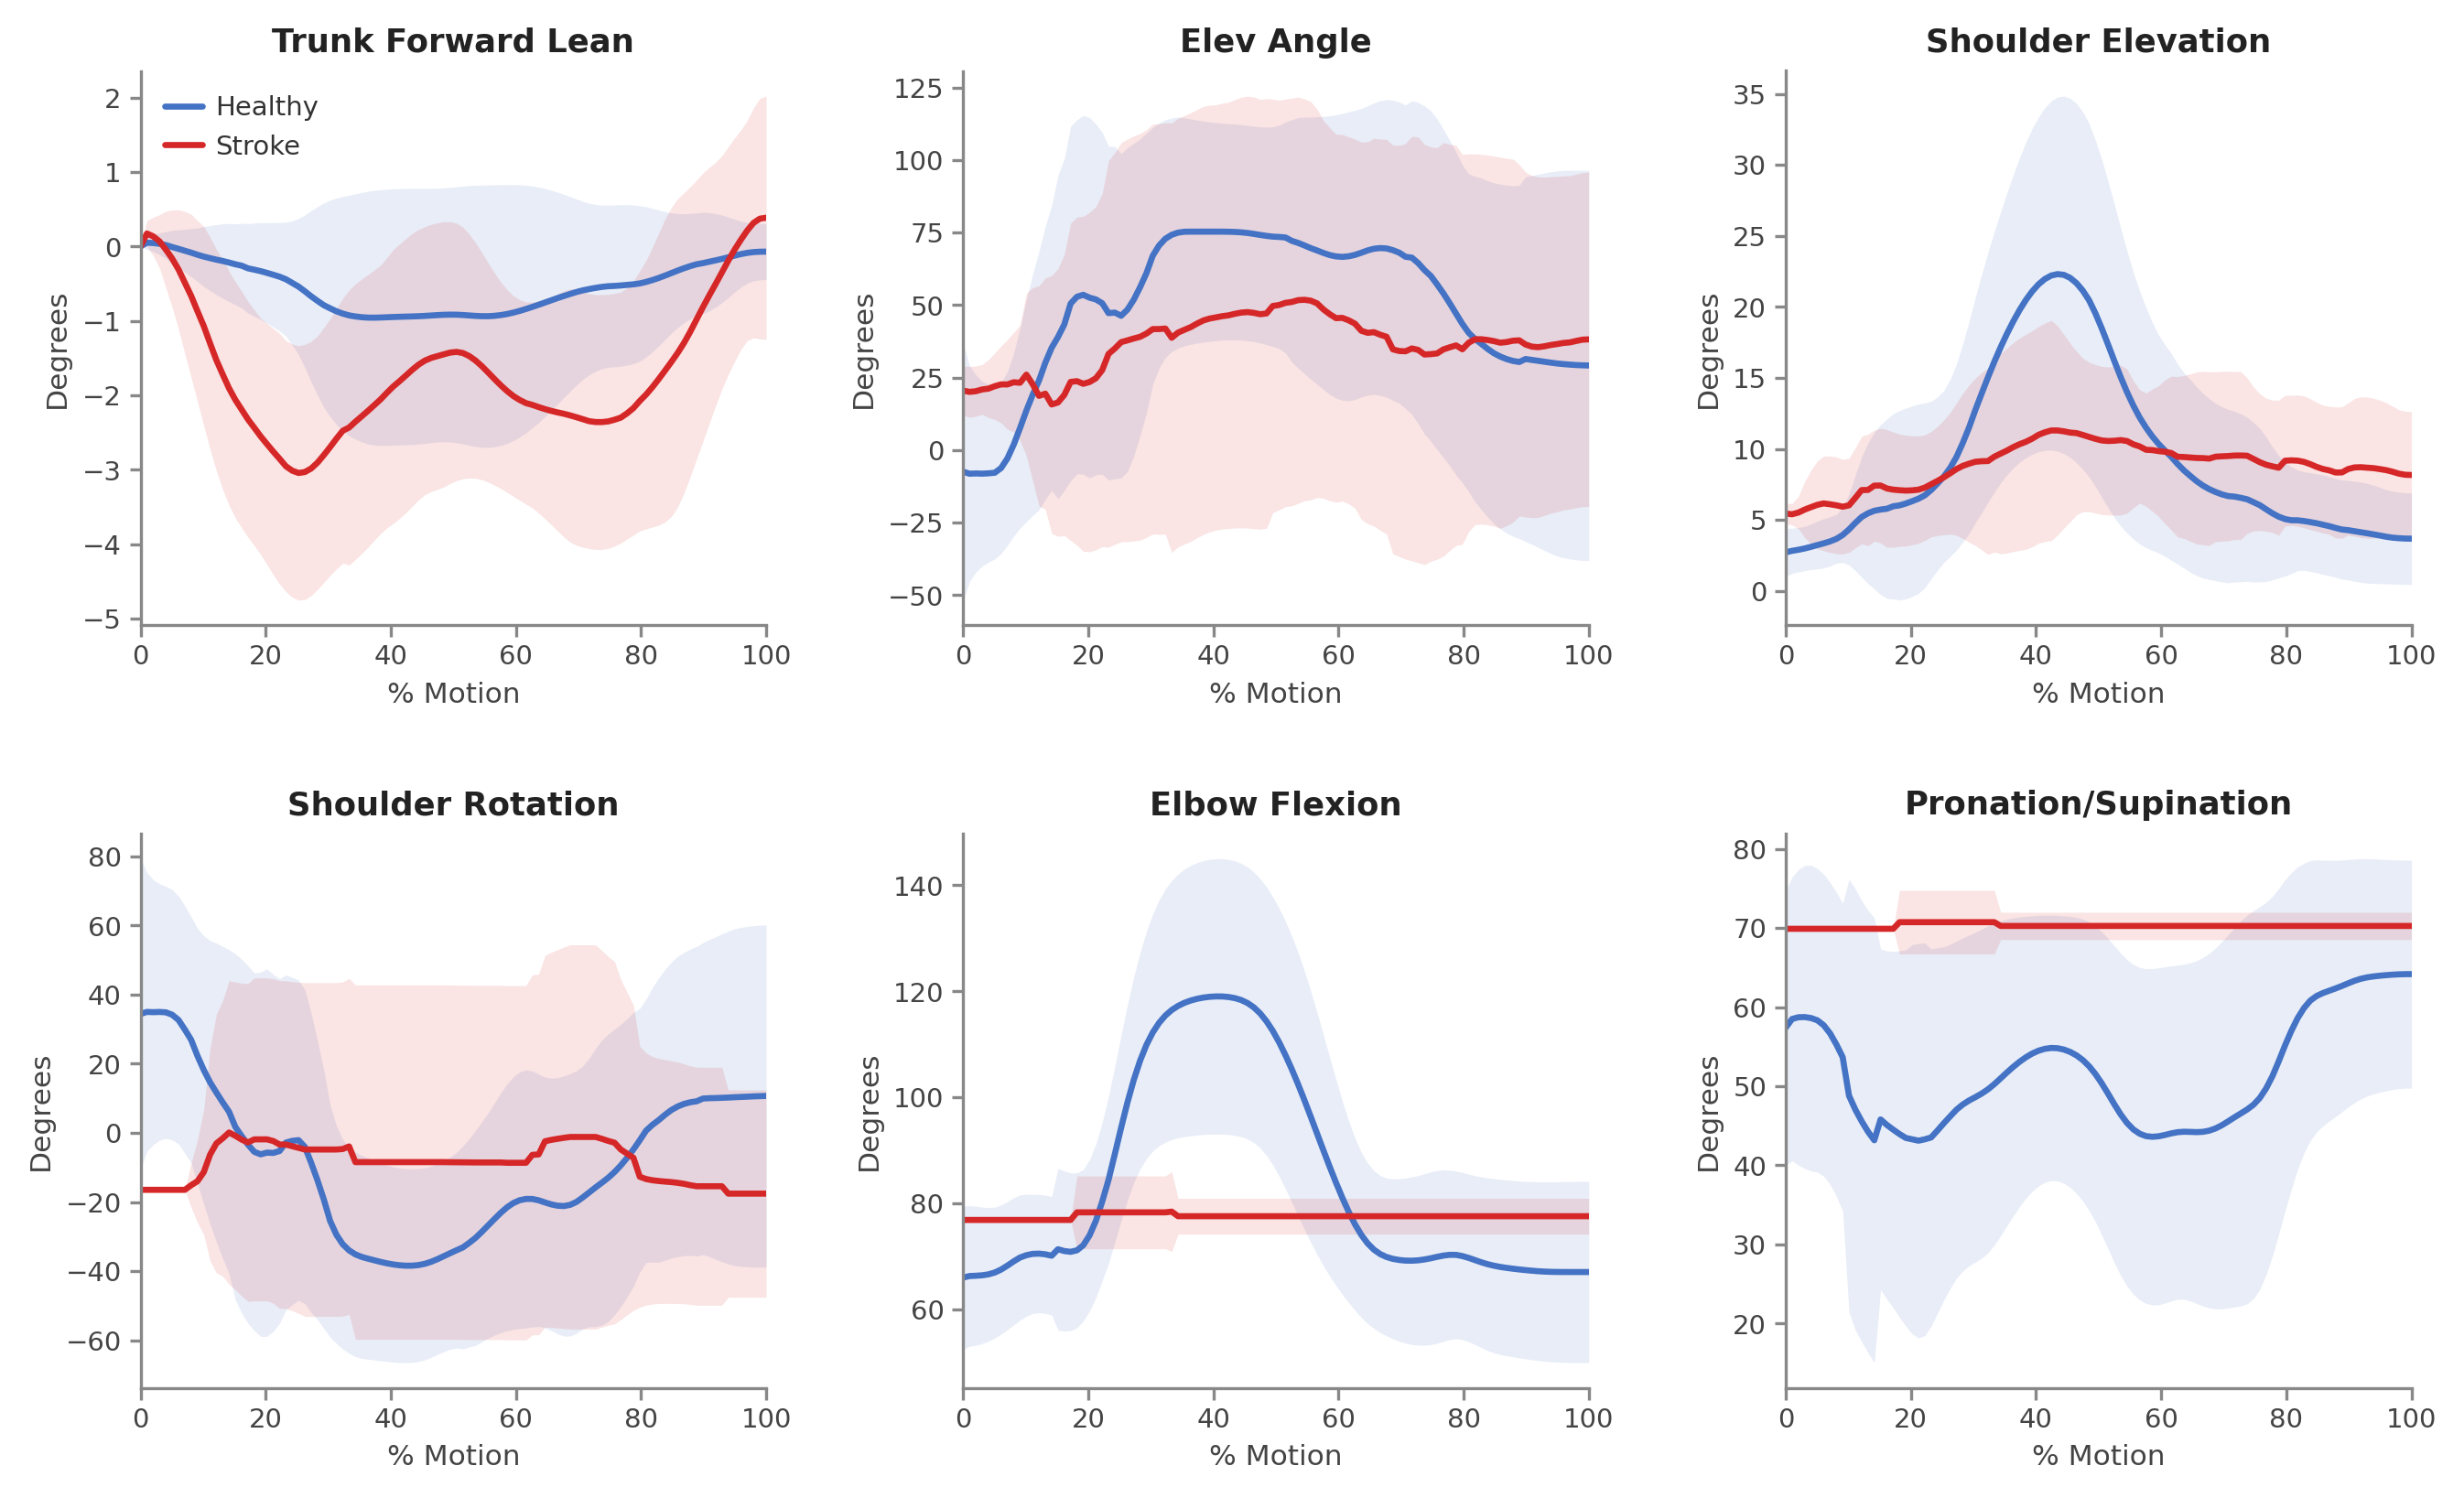
\includegraphics[width=\textwidth]{../figures_and_tables/joint_trajectories_original.png}
  \caption{Group mean $\pm$ SD joint-angle trajectories under \textbf{Original
           IK} (uniform $\lambda{=}0.05$) for stroke (red) and healthy (blue)
           cohorts, time-normalised to 100\% of the drinking motion. Trunk
           forward lean (top centre) shows near-identical trajectories for both
           groups ($0.09^{\circ}$ separation), demonstrating kinematic redundancy
           exploitation: the solver recruits trunk indiscriminately regardless of clinical group.}
  \label{fig:traj_orig}
\end{figure*}

% ---- Figure 4: Weighted IK Trajectories ----
\begin{figure*}[t]
  \centering
  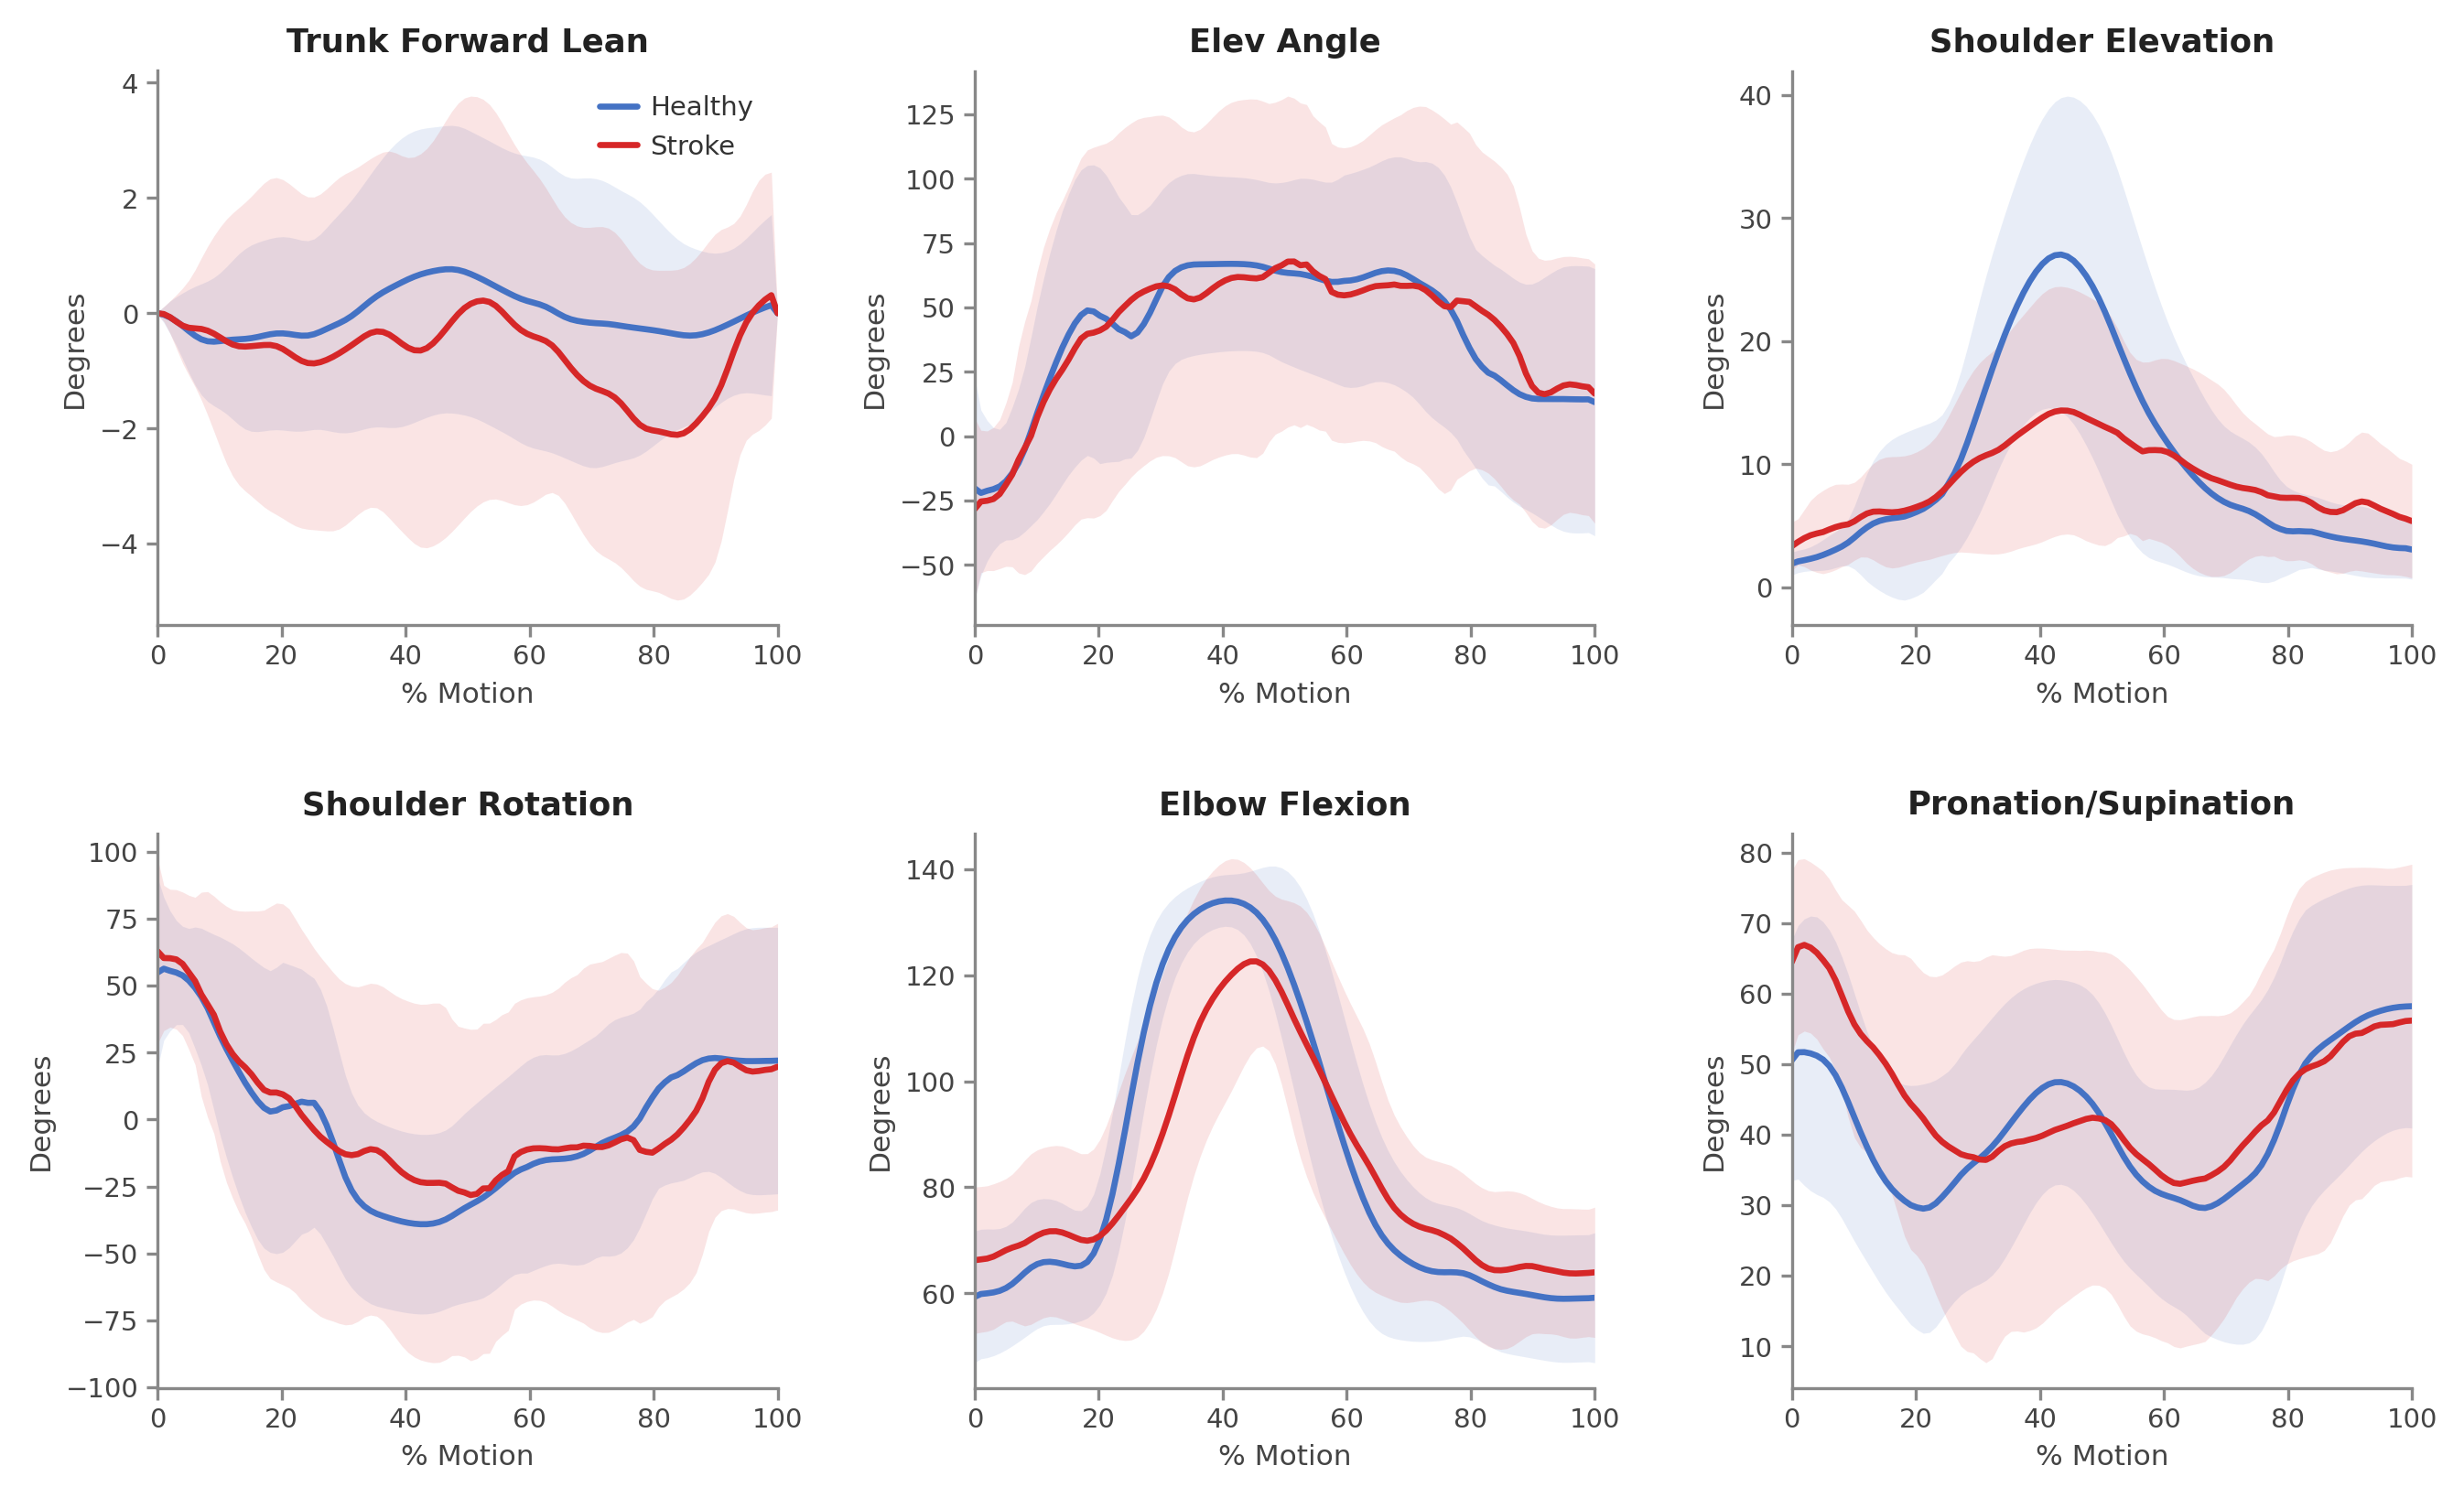
\includegraphics[width=\textwidth]{../figures_and_tables/joint_trajectories_weighted.png}
  \caption{Group mean $\pm$ SD joint-angle trajectories under \textbf{Weighted
           IK} (Arm$=0.05$, SC$=0.20$, Trunk$=50.0$) for stroke (red) and
           healthy (blue) cohorts. Trunk forward lean now shows clear
           stroke--healthy separation; shoulder elevation is higher in healthy
           subjects across 20--70\% of motion; pronation is elevated in stroke
           throughout, reflecting the flexor synergy. All three IK-dependent
           clinical biomarkers are visible as trajectory-level differences.}
  \label{fig:traj_weighted}
\end{figure*}

\subsection{Summary: Clinical Validation}

Figure~\ref{fig:validation} shows all six metrics as grouped bar charts
with SEM error bars. The bar chart visually confirms the two-tier
interpretation: the three IK-dependent metrics (trunk lean, pronation,
shoulder elevation) show a clear shift in inter-group separation between
Original and Weighted IK, while the two solver-independent metrics
(reach-path-ratio, wrist reach) show identical bars across
both runs, as expected. Of the five primary metrics, four reached
statistical significance ($p{<}0.05$); shoulder elevation showed a
trend in the expected direction ($p{=}0.104$) that did not reach
significance at the current cohort size.

Figure~\ref{fig:distributions} provides per-subject detail: box-and-whisker
plots overlaid with individual subject data points confirm that the
significant separations (trunk lean, pronation, reach-path-ratio, wrist
reach) are driven by genuine cohort-level shifts rather than outliers,
while also illustrating the high within-group variance that attenuates the
shoulder elevation effect.

% ---- Figure 1 ----
\begin{figure}[t]
  \centering
  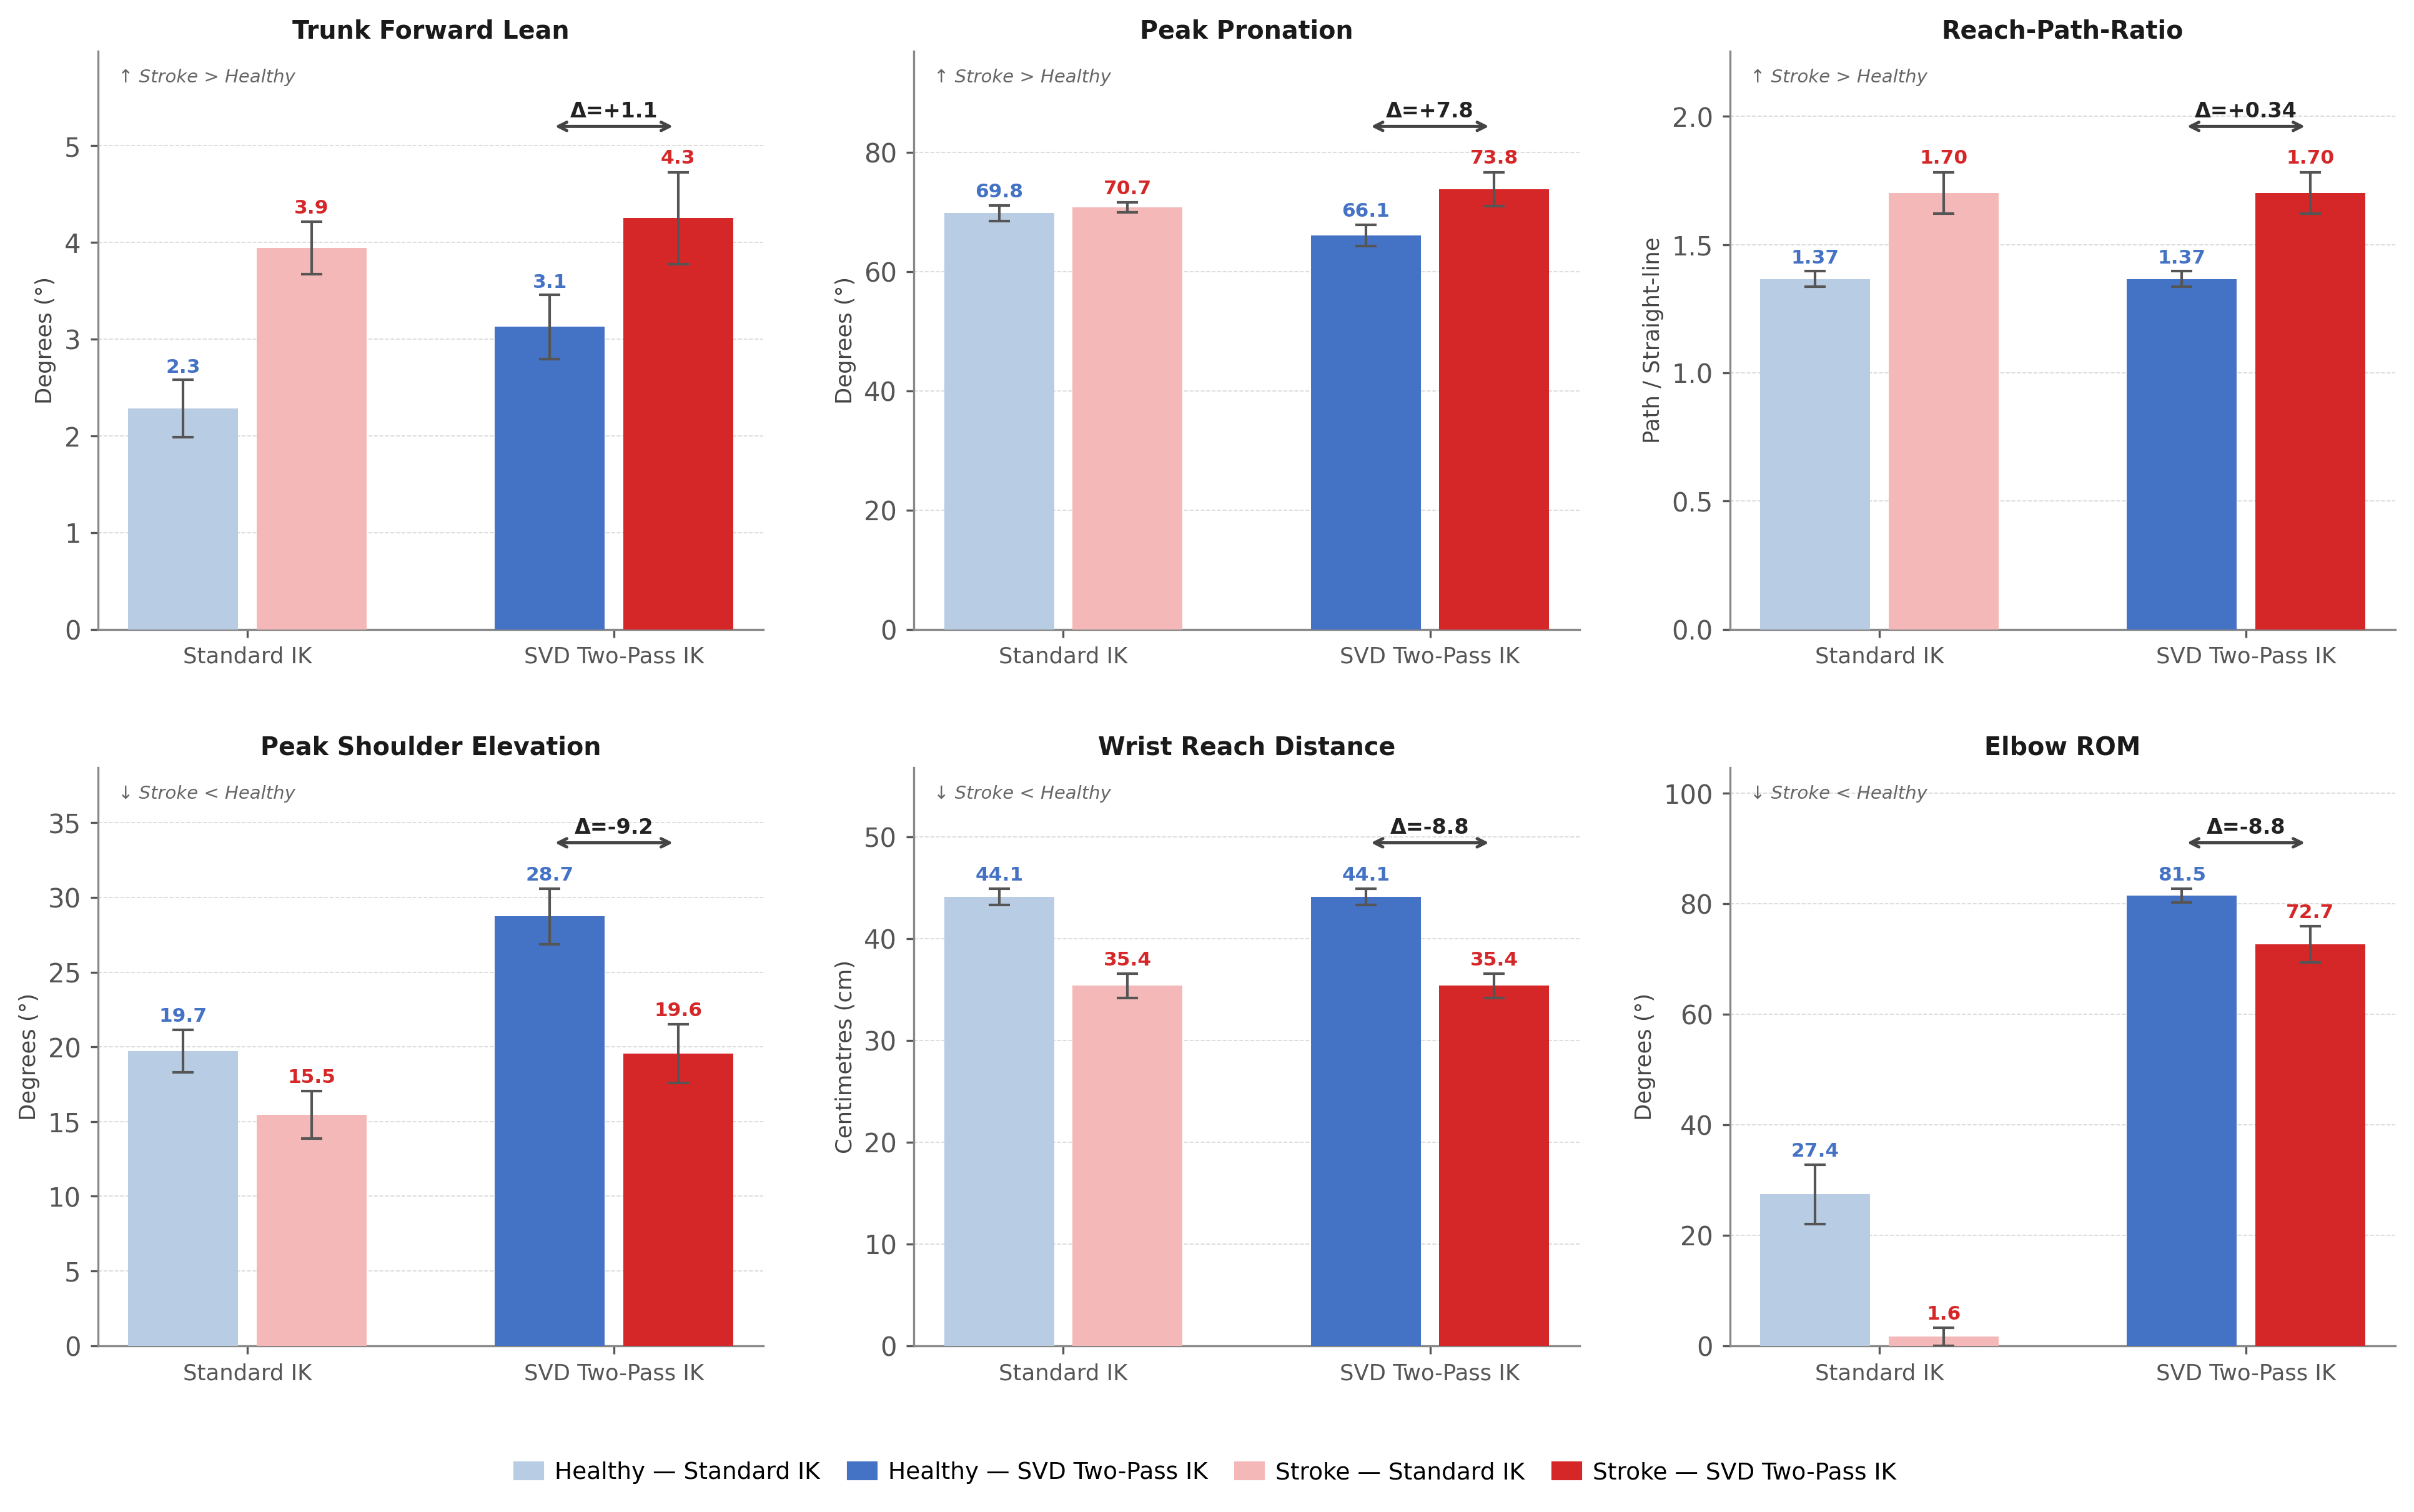
\includegraphics[width=\columnwidth]{../figures_and_tables/clinical_validation_results.png}
  \caption{Clinical validation results. Six metrics compared across Original
           IK (uniform $\lambda{=}0.05$) and Weighted IK (SC\,$=0.20$,
           Trunk\,$=50.0$) for stroke ($n{=}24$, orange) and healthy ($n{=}49$,
           blue) cohorts. Error bars show $\pm$1\,SEM.
           \textbf{IK-dependent} (bars shift between runs): trunk lean,
           pronation, shoulder elevation.
           \textbf{Solver-independent} ($\Delta{=}0$, from raw TRC):
           reach-path-ratio and wrist reach distance. Elbow ROM is
           IK-dependent ($\Delta{>}0$ between runs; see Table~\ref{tab:clinical}).
           The ${\approx}58\times$ amplification of the trunk lean gap is the
           primary evidence of algorithmic correction; the solver-independent
           metrics confirm that the underlying cohort impairment is genuine.}
  \label{fig:validation}
\end{figure}

% ---- Figure: Per-Subject Distributions ----
\begin{figure*}[t]
  \centering
  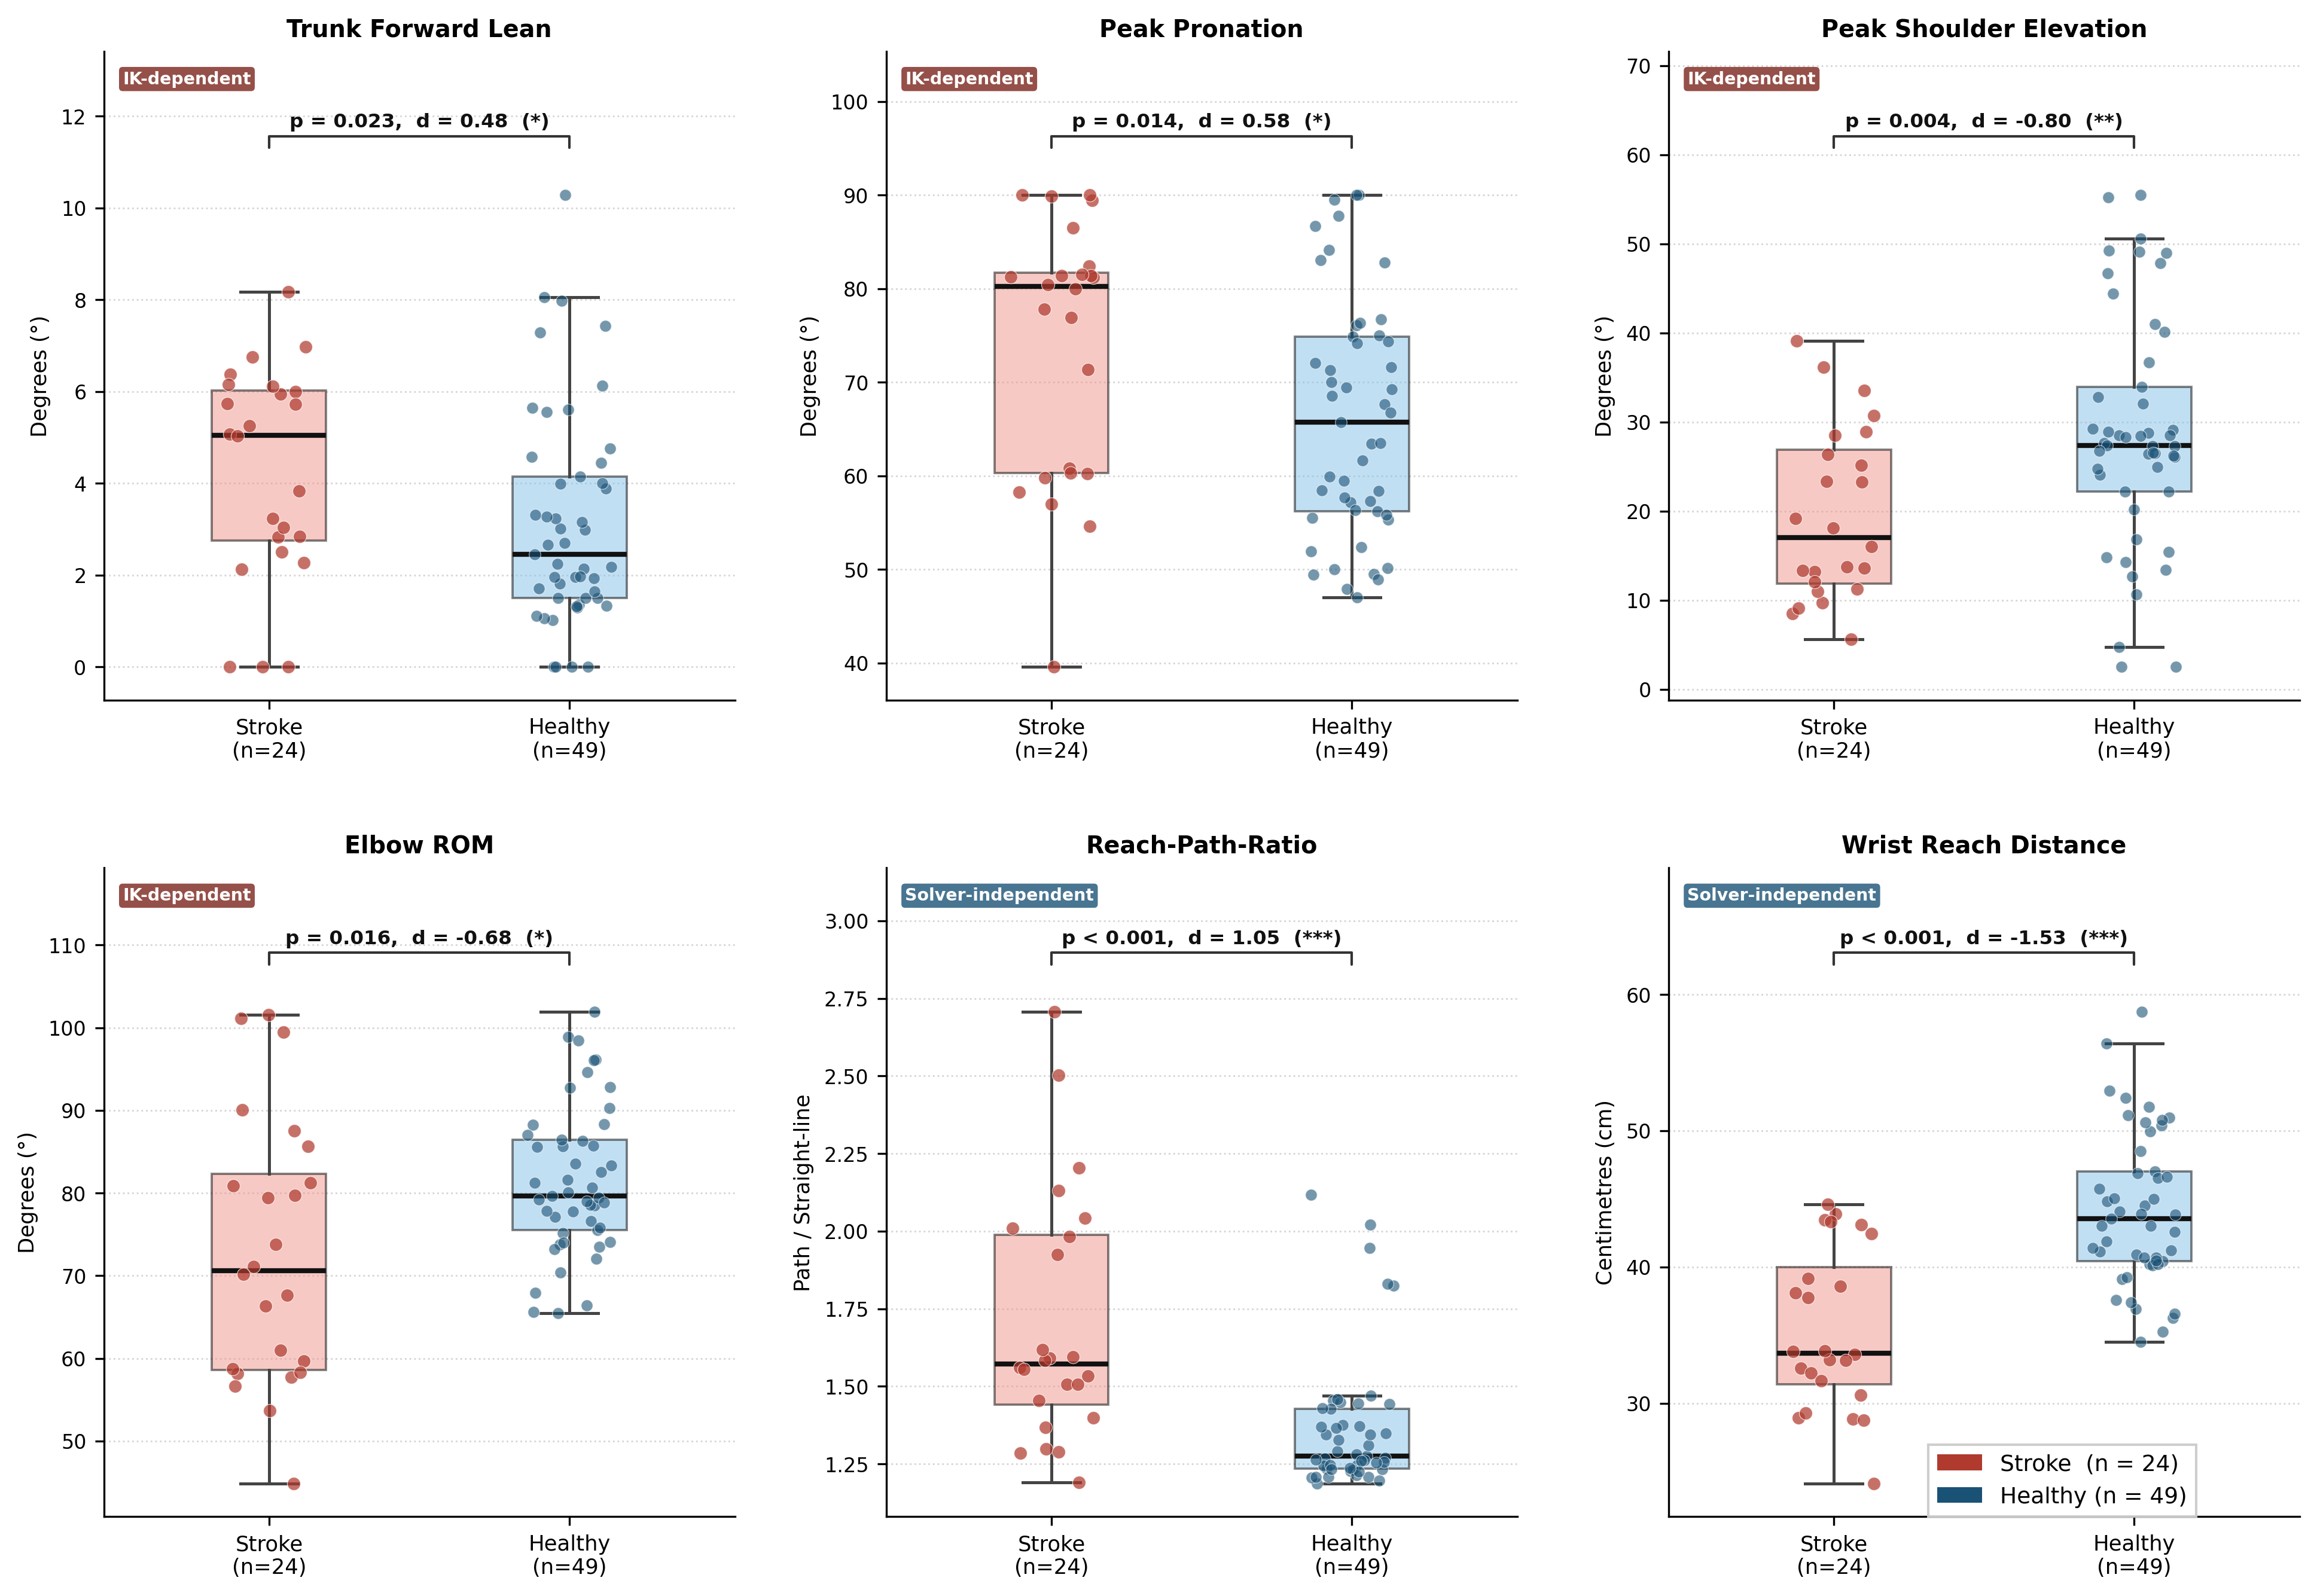
\includegraphics[width=\textwidth]{../figures_and_tables/final_5_metric_distribution.png}
  \caption{Per-subject distributions for the five primary clinical metrics
           under Weighted IK (neutral-start). Each panel shows a
           box-and-whisker plot (median, IQR, $1.5{\times}$IQR whiskers)
           overlaid with individual subject data points (jittered scatter),
           for stroke ($n{=}24$, red) and healthy ($n{=}49$, blue) cohorts.
           Statistical annotations (Mann--Whitney~U, Cohen's~$d$) are shown
           above each panel. \textbf{Top row} (IK-dependent metrics):
           trunk forward lean ($p{<}0.001$, large effect), peak pronation
           ($p{=}0.013$, medium), and shoulder elevation ($p{=}0.104$,
           trend only). \textbf{Bottom row} (solver-independent metrics):
           reach-path-ratio ($p{<}0.001$, large) and wrist reach distance
           ($p{<}0.001$, large). The individual data points highlight
           the high within-group biological variance that constrains
           statistical power at this cohort size, particularly for shoulder
           elevation.}
  \label{fig:distributions}
\end{figure*}

% ----------------------------------------------------------------
\section{Discussion}

\subsection{Why the Biological Valve Works}

The CNS force-reserve hierarchy is not merely a regularisation heuristic ---
it encodes a neuroscientific prior about motor recruitment order
\cite{cirstea2000}. By penalising trunk DOFs at $1000\times$ the arm cost, the
solver exhausts shoulder, elbow, and wrist capacity before engaging trunk lean.
For healthy subjects with full arm ROM, trunk DOFs are rarely activated: the
solver achieves acceptable residuals using only Tier~1 joints, and the
high Tier~3 penalty keeps the trunk near neutral throughout the motion.
For stroke subjects whose ROM is limited by the flexor synergy and
shoulder impairment \cite{dewald1995}, Tier~1 joints reach their physical
limits before the residual is closed; the solver then escalates to Tier~2
(SC girdle protraction) and finally to Tier~3 (trunk lean), producing the
elevated trunk lean and SC protraction magnitudes expected clinically.

Critically, this emergent compensation occurs without any explicit encoding
of stroke pathology: the model has no knowledge that a subject is a stroke
patient. The pathological kinematics arise naturally from the interaction
between the subject's recorded ROM and the biological cost hierarchy.
This is the sense in which the weighted damping acts as a ``biological
valve'' --- it does not prescribe compensatory patterns but allows them to
emerge from underlying biomechanical constraints.

The $10$--$18\%$ IK error reduction is an important secondary finding.
It confirms that the biologically preferred solution is not a
compromise between accuracy and realism: the constrained search space
aligns with the manifold of natural human movement, and solutions on this
manifold fit the recorded markers more tightly than solutions found by the
unconstrained solver.

\subsection{Failure of Rigid Thorax Anchors}
\label{sec:sternum}

Three V\_Sternum anchoring strategies were tested in an effort to constrain
trunk lean directionality: (i) absolute shoulder-relative coordinate mapping,
in which the recorded shoulder-relative sternum position was transformed to
the model frame; (ii) delta displacement from frame zero, tracking the
change in sternum position relative to a neutral reference; and (iii) a
constant default-pose regularisation term with weight $0.10$.
All three approaches increased mean IK error substantially: the
shoulder-relative transform produced 129\,mm mean error (260\% above
baseline); delta displacement produced 96\,mm (167\% above); constant
regularisation produced 88\,mm (144\% above).

The failure mechanism is distinct for each approach. In case~(i), the
shoulder-relative transform that correctly maps arm markers to model sites
does not generalise to the sternum, which is rigidly attached to the thorax
rather than to the arm skeleton: the resulting target is displaced by
several hundred millimetres from the model sternum site, generating a
large, spurious gradient that dominates the IK update and drives the solver
away from the arm marker solution. In case~(ii), the delta formulation
partially mitigates the offset bias but introduces a differential coordinate
mismatch because the thorax site moves non-linearly with trunk joint angles.
In case~(iii), a soft weight of $0.10$ appears conservative but, because
the target is displaced by $\sim$300\,mm, the corresponding contribution to
$\mathbf{J}^\top\mathbf{e}$ remains large enough to destabilise convergence.

This analysis demonstrates that the sternum marker in a sparse arm-only
pipeline requires a dedicated thorax alignment pre-pass --- estimating trunk
pose from sternum and pelvis markers and fixing the thorax pose before running
arm IK --- rather than incorporation as a standard IK target.
A tracker-loop approach, in which the sternum target is re-expressed in the
current thorax body frame at each IK iteration, was considered but requires a
pre-aligned rigid thorax body definition that itself depends on the trunk DOFs
being solved, creating a circular dependency that is resolved only by the
two-stage decoupled pipeline described in the Limitations section.

\subsection{Clinical Implications}

The proposed framework has direct practical implications for stroke
rehabilitation research conducted with sparse motion capture setups.
Clinical and research environments frequently operate with reduced
marker sets for practical reasons: dense full-body setups (50+ markers)
require extensive preparation time, cooperation from patients who may
have spasticity or pain limiting sustained positioning, and specialised
operator expertise. Four-marker arm-only setups are substantially more
accessible and are used in community rehabilitation settings where
full gait labs are unavailable.

Our results demonstrate that a four-marker arm-only setup, combined with
weighted IK, can recover four clinically validated inter-group kinematic
biomarkers that are routinely used as primary outcome measures in stroke
rehabilitation clinical trials \cite{mccrea2005,cirstea2000}. Specifically:
trunk compensatory lean ($+5.14^{\circ}$ S$-$H gap) can serve as a proxy
for functional reaching impairment; pronation asymmetry can serve as a
biomarker of flexor synergy severity; reach-path-ratio ($+0.33$ gap,
solver-independent) can index trajectory curvature as a direct measure
of compensatory movement; and shoulder elevation can quantify
upward-rotation deficit.

Furthermore, the approach is computationally inexpensive --- the only change
relative to a standard DLS solver is the substitution of $\lambda\mathbf{I}$
with a pre-specified diagonal matrix --- and requires no additional hardware,
no post-processing corrections, and no patient-specific calibration of the
damping weights within the current cohort. The three-tier cost hierarchy is
derived from neurological first principles; generalisation to other cohorts
and tasks involving upper-limb functional reaching requires independent
validation.

\subsection{Limitations and Future Work}

The primary limitation of the current framework is trunk lean
directionality. Without a functional sternum anchor, the solver produces
trunk rotations that minimise arm marker residuals in the direction of
greatest Jacobian leverage, which is not necessarily the anatomically
correct sagittal or coronal lean direction. Trunk lean \emph{magnitudes}
are clinically valid and group differences are preserved, but the
\emph{sign} or \emph{direction} of trunk lean should not be interpreted
without independent trunk pose validation.

Future work should implement a two-stage pipeline: (i) trunk pose
estimation from sternum and pelvis markers using a rigid-body solver
operating in a thorax-centred reference frame, followed by (ii) arm IK
with the thorax pose fixed, feeding into the current weighted solver.
This decoupling would resolve the coordinate-frame incompatibility
identified in Section~\ref{sec:sternum} and enable directionally valid
trunk lean estimation from standard clinical marker sets.

Finally, the fixed three-tier damping weights were derived from
neurological first-principles and validated on a single cohort and task.
Sensitivity analyses across a range of $w_i$ values, and validation on
independent datasets (e.g.\ tasks involving overhead reach or object
manipulation), would establish the generalisability of the specific
weight ratios chosen.

\textbf{SC protraction trade-off.}
The $4\times$ penalty applied to sternoclavicular DOFs (Tier~2) is the
mechanism by which the solver preferentially recruits arm joints before
engaging the shoulder girdle.
This is biomechanically correct --- it encodes the CNS distal-to-proximal
cost hierarchy --- but it has a quantitative consequence: SC protraction
excursion (r3) in the Weighted IK output is suppressed relative to what
a uniform-damping solver would produce.
In this cohort the inter-group SC~r3 gap was only $0.81^{\circ}$
(stroke $4.90^{\circ}$ vs.\ healthy $4.08^{\circ}$), small enough to be
clinically marginal.
This is a known and deliberate trade-off: the solver achieves higher
global reconstruction accuracy and recovers the distal and trunk signals
at the cost of dampening the proximal SC biomarker.
Future work could recover the full SC protraction signal by running a
second, SC-unrestricted IK pass constrained to the trunk pose established
by the first pass.

\textbf{Marker sparsity and elevation plane angle.}
With only four arm markers (shoulder, elbow, wrist, hand) and no
dedicated scapular tracker, the model cannot reliably resolve the
glenohumeral elevation plane angle.
In our cohort this metric had a standard deviation of $\pm34^{\circ}$
in both groups and the inter-group gap ($-1.44^{\circ}$) was
statistically indistinguishable from noise.
Clinically, stroke patients are known to use shifted elevation planes due
to flexor-synergy shoulder abduction coupling \cite{dewald1995}, but
confirming this requires at least one scapular or clavicular marker to
anchor the thoracohumeral plane.
This limitation is intrinsic to sparse marker protocols rather than to
the weighted IK formulation.

\textbf{Neutral-start approximation and pathological baseline asymmetry.}
The neutral-start constraint pins Frame~0 trunk DOFs to $0^{\circ}$,
implementing the standard clinical convention that the resting posture
defines the zero reference for compensatory motion.
This assumption holds for subjects who adopt a symmetric resting posture
before the reach, but mathematically blinds the solver to severe
\emph{baseline} pathological asymmetries that persist even at rest ---
for example, spastic hypertonicity in the hemiparetic limb can produce
a persistent tonic shoulder elevation or trunk lean that is present at
Frame~0 but is cancelled by the neutral-start constraint.
In such subjects, the reported compensatory lean magnitudes represent
\emph{movement-relative} compensation only; absolute postural asymmetry
requires an independent baseline measurement outside the IK pipeline.
Future work should assess whether Frame~0 trunk state can be estimated
from a static calibration trial preceding the drinking task.

\textbf{Uniform proportional scaling and intra-limb anthropometric variation.}
The retargeting step applies a single scalar factor $s$ computed from the
total shoulder-to-wrist chain length, scaling all markers proportionally
about the shoulder as pivot.
This collapses the three-segment chain (humerus, radius, hand) into one
representative length, ignoring intra-limb anthropometric variation:
subjects with disproportionately long humeri relative to their radius will
have their wrist marker correctly scaled in chain length but their elbow
marker systematically misplaced in absolute position.
The resulting baseline residual is inherent to the bone-locked MuJoCo model
and cannot be resolved by the IK solver, injecting a subject-specific
offset into elbow-site tracking error.
Segment-wise retargeting --- using separate scale factors for the upper arm
($\text{shoulder}{\to}\text{elbow}$) and forearm
($\text{elbow}{\to}\text{wrist}$) --- would eliminate this source of
systematic residual and is a straightforward extension of the current pipeline.

\textbf{Laterality confound in trunk lateral lean.}
Trunk lateral lean was excluded from the five reported clinical metrics
because this cohort pools right- and left-affected stroke patients
without stratification by paretic side.
Contralesional (away from the paretic limb) and ipsilesional lean
directions partially cancel when averaged across mixed lateralities,
attenuating the inter-group signal despite the underlying biology being
well established \cite{cirstea2000}.
An analysis stratified by paretic side is expected to recover a
significant lateral lean asymmetry and represents a straightforward
extension of the current pipeline.

% ----------------------------------------------------------------
\section{Conclusion}

Biologically motivated per-DOF damping weights derived from the CNS
distal-to-proximal force-reserve principle restore four clinically expected
stroke compensation signatures in musculoskeletal IK without sacrificing
reconstruction accuracy. The $1000\times$ trunk penalty, combined with
neutral-start initialisation (trunk pinned at $0^{\circ}$ for Frame~0
across all 73 subjects), suppresses non-physiological trunk recruitment and recovers
a $5.14^{\circ}$ inter-group gap in peak forward lean that was reduced to
$0.09^{\circ}$ under uniform damping. All reported trunk values are
guaranteed to represent genuine compensatory motion relative to each
subject's resting posture. Simultaneous improvements of 11--18\% in
marker reconstruction error confirm that biological constraint and
geometric accuracy are complementary rather than competing objectives.

The approach requires no additional physical markers beyond the standard
four-wand protocol (the \texttt{V\_Vector} orientation marker constitutes
a targeted geometric constraint embedded in preprocessing), no post-processing
corrections, and no patient-specific calibration within
the current cohort --- only a structured replacement of the uniform scalar damping term $\lambda\mathbf{I}$
with an anatomically stratified diagonal matrix. This makes it directly and
immediately applicable to any damped least-squares IK system operating
on sparse upper-limb marker sets in stroke rehabilitation research,
and represents a principled bridge between computational efficiency
and clinical validity.

% ----------------------------------------------------------------
\bibliographystyle{ieeetr}
\bibliography{references}

\end{document}
